\documentclass{article}
\usepackage{graphicx} % Required for inserting images
\usepackage{amssymb}  
\usepackage{amsmath}
\usepackage{float}
\usepackage[document]{ragged2e}
\usepackage{graphicx}
\usepackage{pst-solides3d}
\pagestyle{empty}
\usepackage{exscale}
\usepackage{textcomp}
\usepackage{enumerate}
\usepackage{tabularx}
\usepackage{geometry}
\usepackage{amsfonts} 
\usepackage{listings}
\usepackage{tensor}
\geometry{legalpaper, margin=1in}
\usepackage[table]{xcolor}
\setlength{\arrayrulewidth}{0.5mm}
\setlength{\tabcolsep}{18pt}
%\renewcommand{\arraystretch}{2.5}
\usepackage{blindtext}
\usepackage{subcaption}
\usepackage{hyperref}
\hypersetup{ colorlinks = true,
            linkcolor = blue,
            filecolor = magenta,
            urlcolor = cyan}   
\graphicspath{{./maths project}}
\usepackage [english]{babel}
\usepackage [autostyle, english = american]{csquotes}
\MakeOuterQuote{"}

\usepackage{color}
\newcommand{\com}[1]{{\sf\color[rgb]{0,0,1}[#1]}}
\usepackage[normalem]{ulem}  % \sout{old text} for strikeout
\newcommand{\new}[1]{{\color[rgb]{0.9,0,0}#1}}
\newcommand{\old}[1]{{\color[rgb]{0.7,0,0.7}\sout{#1}}}
\usepackage{tikz}
\usepackage{tikz-cd}
\usetikzlibrary{matrix, calc, arrows}
\usetikzlibrary{shapes.misc}
\newcommand*\cancel[2][thin]{\tikz[baseline] \node [strike out,draw,anchor=text,inner sep=0pt,text=black,#1]{#2};}  
\usepackage{biblatex}
\addbibresource{references.bib}
\newcommand{\be}{\begin{equation}}
\newcommand{\ee}{\end{equation}}
\newcommand{\bea}{\begin{eqnarray}}
\newcommand{\eea}{\end{eqnarray}}
\newtheorem{theorem}{Theorem}[section]
\newtheorem{definition}[theorem]{Definition}
\newtheorem{example}[theorem]{Example}
\newtheorem{proposition}[theorem]{Proposition}


\title{Topological Data Analysis}
\author{Isaac Gonzales}
\date{November 2023}

\begin{document}

\maketitle
\pagenumbering{roman}
\newpage

\tableofcontents

\clearpage

\pagenumbering{arabic}
\section{Introduction}
Extracting qualitative analysis and predominant features of a dataset and to create a story is the aim for any data analyst, data scientist, statistician and anyone curious. With the rapid advancement of technology, data is constantly being collected in a various formats, resulting in datasets that are noisy and may be higher dimensional that the use of standard statistical tools to analyse become redundant\cite{IntroTDADATAscientists}. This increased demand for methodologies to analyse massive datasets has led applied mathematicians to develop tools within topology, a branch of mathematics concerned with the structure and shape. Topology is able to summarise topological spaces to their fundamental geometric features regardless on the chosen metric or coordinates of the space\cite{CarlssonAMS}: features such as path-connected, connected, compact, loops, voids and higher dimensional equivalences \cite{Hatcher}\cite{HSchenckAlgebraicFound}. This allows for these topological properties to arise, that were otherwise hidden by complicated or noisy data, to be used to classify an object. Topological data analysis, TDA for short, is a topological lens into the attempt of obtaining qualitative information from a data set. As its name indicates, TDA applies concepts from algebraic topology to analyse data sets. TDA can be viewed as a field that is a blend of data analysis and science, statistics, algebraic topology and computational geometry. \cite{NINARoadmap}\cite{smith2020topological}. \\ 
The first half of this paper will involve the introduction of the definitions,theorems, and concepts within algebraic topology and homology that are required for TDA. Algebraic topology combines linear algebra and topology by using methods in linear algebra to compute geometric features of shapes and spaces\cite{AZComputePH} \cite{Maleti__2016} \cite{AZadvances}. Homology, a functor in algebraic topology, is only concerned with dominant intrinsic geometric features of connectedness, loops, voids, and higher dimensional equivalences. The main method in TDA is persistent homology and heavily rely on the concepts defined in the preliminary chapter. The homology functor maps simplicial complexes to $R$-module. Essentially, homology translates a geometric object into an algebraic object. Persistent homology provides a way to unveil the qualitative, a tool to compute them, and confirms robustness of those features \cite{smith2020topological}. Simplicial complexes can be thought as spaces constructed by building blocks defined where one of these building blocks is defined a as $k$-simplex. Simplicial complexes can be defined abstractly and geometrically. Both will be introduced as the geometric realization of a simplicial complex aids in the understanding of the abstract definition. If we think back to the early years of mathematical education in school one of the first concepts taught in geometry was shapes. The study of shapes can be dated back to the curious minds of the ancient Egyptian and Greek philosophers and mathematicians. Most notably, Euclid of Alexandra (300 B.C.) complies the works of his own and his predecessors into the mathematical bible: 'Euclid's Elements'. 'Euclid's Elements' consists of 13 books covering topics and axioms in geometry, algebra and number theory that still persist and remain unchanged. The beloved triangle: the shape with 3 sides, 3 corners and 3 angles that have a sum of 180 degrees. The simple Pythagorean equation $a^2 + b^2 = c^2$ relating the edges of a right angled triangle. The ratio of the edges of a triangle beautifully described by trigonometric functions. In two dimensional Euclidean space, every simple polygon admits a triangulation and any triangulation of a simple polygon with $n$ vertices consists of exactly $n-2$ triangles. However, this property cannot be extended to their three dimensional counterpart, not every triangulation of a polyhedron consists of the same number of tetrahedron (three dimensional triangle equivalent). The idea of triangulation of a polygon is analogous to the idea of a simplicial complex of a space $X$. A simplicial complex is the decomposition of a space by its $k$-simplicies; the $k$-th dimensional triangle equivalences. One of the first topological invariant properties we will see is the Euler characteristic. A topological invariant property is a property that remains unchanged under homeomorphisms (bijective, continuous functions between topological spaces). If two objects are topologically the same they have the same Euler characteristic, a property based on a relationship between the number of edges (E), vertices (V) and faces (F). The Euler characteristic is given by the formula $\chi = V - E + F $ , and is the same for all shapes whose boundaries are composed of the same number of connected pieces. 
For all simple polygons the Euler characteristic is one. By using triangulation one can compute the Euler characteristic. For the three dimensional case, any simple polyhedral, the Euler characteristic is 2. This can be demonstrated by removing one face (with Euler characteristic of 1) and deform the remaining figure onto a plane by "stretching" (a continuous deformation) resulting in a simple polygon with a Euler characteristic of 1. By adding the Euler characteristic of the removed face, we have that the simple polyhedral has a Euler characteristic of 2.
to apply the homology functor by turning a geometric problem in to an algebraic one. The persistence module and homology, introduced by Edelsbrunner, Letscher, and Zomorodian \cite{EdelTopPersist} and later Carlsson and Zomorodian \cite{AZComputePH} showed that a persistence has the structure of a graded module over a principal ideal domain and that persistent homology assigns this persistence module to a filtered simplicial complex \cite{HSchenckAlgebraicFound}. Many advancement in TDA has been made and found successful applications in medicine \cite{DEWOSKIN2010157}, material science \cite{https://doi.org/10.1002/jcc.23816}, robotics \cite{TOPTrajeFlorian}, image processing \cite{CSurfaceDataChung}, dynamical processes \cite{Maleti__2016} and biology\cite{CarlssonTDAappli}.

The second half of this paper will continue to discuss how to apply the TDA pipeline to time series of dynamical systems and the application to financial data. One can defined a dynamical system as a system in which an object evolves over time. There are many dynamical systems that we encounter in our day to day lives. As a child, a popular pastime was to go to the local playground, race to the swings and swing to the heights. The swinging motion can be modelled simply as a swinging pendulum; a ball on a string where the position of the ball is projected and defined by a set of rules such as a function. There are many factors that dictate the motion of the swing such factor are the mass of the person; whether there are drag forces; the material attaching the seat to the frame; whether the person is using their legs to swing or standing on the seat and use a pumping action to drive the swing up. Each additional factor to the mathematical model increases its complexity to define accurately. It is not always possible to have an exact and explicit mathematical description of a dynamical system as most are chaotic. So one has to formulate a mathematical model to approximate the system by observing its variables. The system is described by its variables at a given time and this is defined as the state of the system that lives in a space. An observation functions acts a rule in how the state of a system evolves. Most data is observed as time progresses.   The aim of Takens' Embedding Theorem is to reconstruct an attractor of a dynamical system where an attractor is the space in which most of the states of a dynamical system evolve to.

\section{Preliminaries}
Human's evolutionary ability for pattern recognition is a survival instinct inherited from our ancestors who had to differentiate prey from predator or poisonous plants from healthy one. Despite the fact the need to survive in the way that our ancestors did has changed, we cannot help but seek for patterns and structure in the information we receive. However, survival is still determined by the successful decisions we make. \\

Finding shape, patterns and correlations embedded in data is not a new concept but the ability to identify such features in the ever growing and noisy data becomes a challenge. The development of TDA , a dimensional reduction technique, maps data from its original high-dimensional space to a low-dimensional space that it is easier to understand and visualize.

This chapter will cover the necessary definitions and theorems in algebraic topology and homology. This will form the basis for understanding persistent homology, a methodology used in TDA. The fundamental objective of the TDA process, is to create a filtration of simplicial complexes from the dataset using a varying parameter and observe the homology groups as the simplicial complex evolves. Majority of the definitions for the modules chapter are from \cite{HSchenckAlgebraicFound} and for simplicial complexes and homology Hatcher's book Algebraic Topology \cite{Hatcher}, resort for further in-depth proofs and examples.
\subsection{Algebra: Modules}
First, we will introduce notions of rings and modules as these are the generalised algebraic objects used in homology theory. In many undergraduate literature, $\mathbb{Z}$ coefficients used for simplicial chains and homology groups and so have abelian group structures. In this paper, we will stick to the generalisation and use $R$ to denote a commutative ring with unity.
\begin{definition}
Let R be a ring. A \textbf{R-module} M over  R is an abelian group, together with a scalar multiplication $R \times M \to M$ such that for all $r, r' \in R$ and $m, m' \in M$ we have,
\begin{itemize}
    \item $r(m + m') = rm + rm'$,
    \item $(r + r')m = rm + r'm$,
    \item $r(r'm_1) = (rr')m$,
    \item $1.(m) = m$,
    \item $0.(m) = 0$.
\end{itemize}
\end{definition}

\begin{example}Examples of rings $R$
\begin{itemize}
    \item Every vector space over a field $k$ is a $k$-module
    \item Examples of fields are $\mathbb{Q}, \mathbb{R}, \mathbb{C}, \mathbb{Z_p}$ where $p$ is prime
    \item Every group is a $\mathbb{Z}$-module
\end{itemize}
\end{example}
An $R$-module M is called \textbf{free} if it has a basis. That is, if there exist a set $S = {m_1, ..., m_n} \subseteq M$ which generates $M$ and is $R$-linearly independent i.e. for any element $m \in M$ can be uniquely expressed as
\be
m = \Sigma ^{n}_{i=1} r_i m_i ,
\ee
for some coefficients $r_i \in R$. The generating set does not necessarily need to be finite but for persistent homology and in this paper the algebraic object are computed from discrete finite point clouds and so the definition for finite $R$-modules will suffice. If a free $R$-module M has a basis of size n, M can be constructed as a direct sum of n copies of R \cite{HSchenckAlgebraicFound}. 

\begin{definition}
Let $M$ and $N$ be $R$-modules. Then a map $f: M \to N$ is called an \textbf{R-homomorphism} if it is $R$-linear i.e. for all $r \in R$ and $m,m' \in M$
\begin{itemize}
    \item f(m+m') = f(m) + f(m'),
    \item f(rm) = rf(m)
\end{itemize}
\end{definition}

\begin{example}
    \begin{itemize}
        \item If R is a field, then an $R$-homomorphism is an (R)-linear transformation
        \item If $R = \mathbb{Z}$, then an $R$-homomorphism is a group homomorphism of abelian groups.
    \end{itemize}
\end{example}
\begin{definition}A ring $R$ is called graded if there exists a family of subgroups ${R_i}_{i\in \mathbb{Z}}$ such that
decomposition of abelian groups,
\be
R \cong \bigoplus_{i}R_{i}, i\in\mathbb{Z}.
\ee the decomposition of abelian groups.
\end{definition}

\begin{definition}
A module $M$ over a graded ring $R$ is called a \textbf{graded R-module} if there exists a family of subgroups ${M_i}_{i\in \mathbb{Z}}$ of $M$ such that,
\be
M \cong \bigoplus_{i}M_{i}, i\in \mathbb{Z},
\ee is a module equipped with a direct sum decomposition of abelian groups.
\end{definition}

In mathematics there are many 'fundamental theorems'; the theorem introduced in this section describes the structure of finitely generated modules over a PID (principal ideal domain). A PID $R$ is an integral domain, a ring without zero divisors, such that every ideal in R is principal i.e generated by a single element. An ideal in a ring $R$ is a subring $I \subseteq R$ such that if $a \in I$ and $r \in R$ then $ar$ and $ra$ belong in $I$  \cite{SYMONDS2007408structure}.
\begin{example} Examples of PIDs

\begin{itemize}
    \item All ideals of $\mathbb{Z}$ are principal.
    \item Any field $k$ and the polynomial ring $k[x]$ are PIDs. Any ideal in $k[x]$ has the form $<f(x)>$.
\end{itemize}
\end{example}
The ring of polynomials $k[x]$ can be thought as a $k$-vector space, $V$, equipped with a $k$-linear transformation $T: V \to V$. 
Before we state the structure theorem for $R$-modules over a PID, we need a few definitions.
\begin{definition}Let $M$ be an $R$-module, $R$ a PID. For $m \in M$, the annihilator of $m$ is,
\be
Ann(m) = \{r \in R : rm = 0\}
\ee
\end{definition}
\begin{definition} Let $M$ be a module over a PID $R$. The torsion submodule $T(M)$ is defined as,
\be
T(M) = \{m\in M : \text{there exists}   r\neq 0, r\in R s.t ra=0 \} 
\ee
\end{definition}
Every free module is torsion-free.
\begin{theorem}(Structure Theorem for Principal Ideal Domains) Let M be a finitely generated $R$-module where R is a PID. Then M is isomorphic to a direct sum of cyclic $R$-modules
\be
M \cong R^{l} \oplus (\bigoplus^{m}_{i=1} R/(n_i)),
\ee
for unique $l\geq 0$, unique $m\geq 0$ and unique $n_i$ up to multiplication by a unit in $R$ with each $n_i > 1$ and $n_{i+1}|n_i$ for $1\leq i \leq m-1$ all determined by M.
\end{theorem}
The algebraic invariant objects in persistent homology are modules over $k[x]$ with the addition that they are $\mathbb{Z}$ graded rings \cite{HSchenckAlgebraicFound}.
The structure theorem can be adapted to finitely generated graded $R$-modules.
\begin{theorem}Let M be a finitely generated graded $R$-module where R is a PID. Then $M$ is isomorphic to a direct sum of cyclic $R$-modules,
\be
M \cong R^{l} \oplus (\bigoplus^{m}_{i=1} R/(I_i)),
\ee
for unique $l\geq 0$, unique $m\geq 0$ and  $I_i$ factors unique up to multiplication by a unit with each $I_i > 1$ and $I_{i+1}|I_i$ for $1\leq i \leq m-1$ all determined by M.
\end{theorem}
$R^{l}$ denotes the direct sum of $l$ copies of the PID $R$. This direct sum is a finite free $R$-module component of the decomposition. Denote $T = \bigoplus^{m}_{i=1} R/(I_i) $ to be a finitely generated torsion $R$-submodule component of the decomposition. 
For $R$ a PID, an $R$-module $M$ is torsion if ann($m$) $\neq 0$ for all $m \in M$. 
The structure theorem for finitely generated graded $R$-modules over a PID $R$ provides an algebraic decomposition of an algebra to understand its structure.
\begin{example} Consider the pair $V$ and $T: V \to V$ where $V$ is a finite dimensional $k$-module and $T$ is a linear transformation. Denote the pair by $M$. Recall that this is a $k[x]$-module. $k[x]$ is a $\mathbb{Z}$ graded module. This graded condition results in the ideals $<f(x)>$ to be monomials $<x^{i}>$ \cite{HSchenckAlgebraicFound}. In chapter 4 the structure theorem for persistent modules will be introduced and this will provide a way to classify the homological invariants of a point cloud.
\end{example}
\subsection{Simplicial complexes} \label{Simplicial Complexes}
The TDA process starts with a dataset in which we want to the data to be in the form of a point cloud. A point cloud is a discrete finite subset $X \subset \mathbb{R}^n$. In chapter 5 we will encounter time series datasets that do not come presented in the form of a point cloud, by applying Taken's embedding theorem and the sliding-window method, one can then obtain the desired form. The aim is to study the topological features of the simplicial complex constructed from the point cloud dataset by using computational topology and homology tools. Simplicial complexes are crucial topological spaces in algebraic topology, enabling the translation of topological questions into algebraic problems through the study of homology groups associated with these complexes. 
To build a simplicial complex we need building blocks called simplices. Simplicies can be thought of as generalisations of triangles for higher dimensions and thus we can 'triangulate' a topological space by gluing simplices together. \hfill\break
\begin{definition} Let $V = \{v_0,...,v_n\}$, be a set of vertices. A \textbf{k-simplex} is an unordered collection of $k+1$ distinct vertices.
\end{definition}

This definition provides a purely combinatorial notion of a simplex. We can also define a $k$-simplex in geometric terms. 
\begin{definition}The standard geometrical $\textbf{k-simplex}$ $\Delta ^{k} \subset \mathbb R^{n+1}$ with the standard basis ${e_0, e_1, .., e_k}$ as its set of vertices is defined as, \\
\be
\Delta ^{k} = \{{ (t_0, t_1, ..., t_k) } \in \mathbb R^{n+1} :\[ \sum_{i=0}^{k} t_i =1, {t_i} \geq 0,  \forall {i}\}\]
\ee
\end{definition}

An $k$-simplex is the smallest convex set in an Euclidean space $\mathbb R^{n}$ containing $k+1$ linearly independent points \textit{$v_0, v_1,...,v_k$}. The points \textit{$v_i$} are the vertices of the simplex, and the simplex is denoted by [\textit{$v_0, v_1,...,v_k$}].\hfill\break
In other words, an $n$-simplex encloses a \textit{n}-dimensional space between $n+1$ connected vertices. The geometric realisation for $k$-simplices are shown schematically in Fig.\ref{fig: Schematic diagram of an n-simplex for n = 0,1,2.}.\\

\begin{figure}[h!]
    \centering
    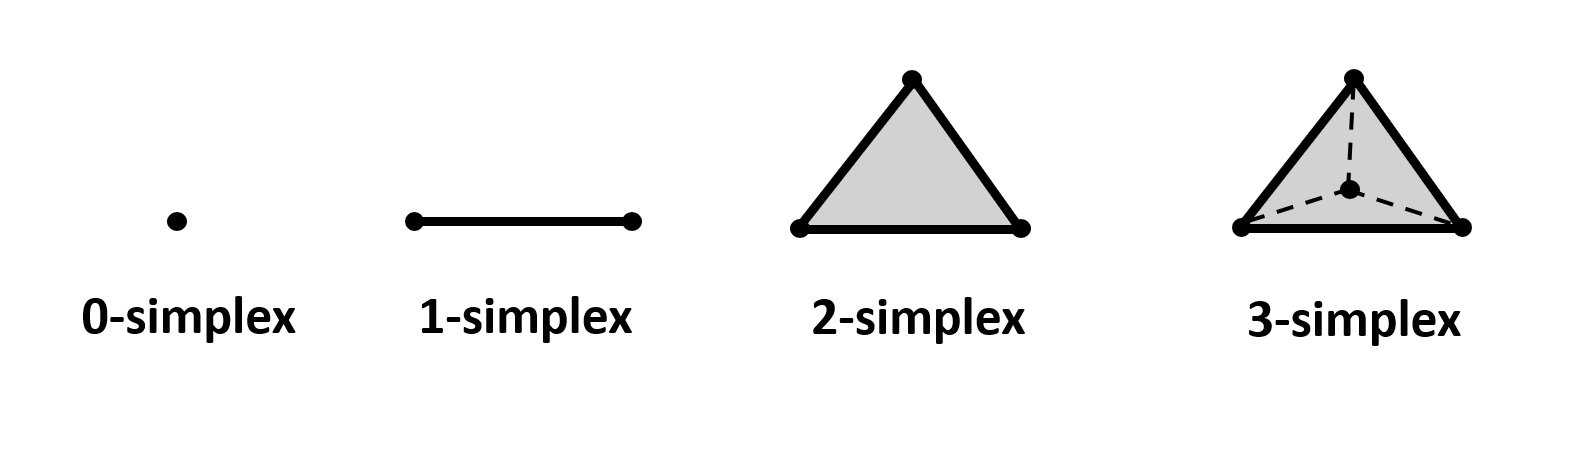
\includegraphics[width= 15cm, height = 4cm]{Simplices.png}
    \caption{Geometric visualisation of n-dimensional simplices for $n = 0,1,2,3$. $0$ simplices are vertices, $1$-simplices are edges, $2$-simplices are triangles, and $3$-simplices are tetrahedra. Simplices are generalisations of triangles in high dimensions.}
    \label{fig: Schematic diagram of an n-simplex for n = 0,1,2.}
\end{figure}

\begin{definition} A \textbf{face} of an $n$-simplex {$v_0, v_1,...,v_n$} is an $n-1$ simplex {$v_0, v_1,...,\hat{v}_i,...,v_n$} where the vertex $v_i$ is deleted. \end{definition}

In Figure.\ref{fig: Schematic diagram of an n-simplex for n = 0,1,2.},to obtain a 0-simplex, remove a vertex (along with its adjacent edge) from a 1-simplex. Repeat process to an $n$-simplex to obtain an $(n-1)$-simplex. 
\begin{definition} If the vertex set V has a choice of a total order on its vertices then an \textbf{orientation} on a $k$-simplex is a total order of its vertices. The orientation of a simplex is dependent on the choice of order on its vertices. The 0-simplex only has one unique choice (as it is a single vertex) and every other $k$-simplex for $k>0$ has two non-equivalent orientations.
\end{definition}
\begin{definition}An \textbf{oriented} $k$-simplex is a simplex with a choice of orientation.
\end{definition}
\begin{definition}An ordered/oriented \textbf{simplicial complex} is a pair $(V,\Sigma)$, where V is a totally ordered finite set and $\Sigma$ is a family of non- empty subsets (simplices) of V denoted by $\sigma = [v_0,...,v_k] $ such that if $\sigma \in \Sigma$ and $\sigma' \subseteq \sigma$, then $\sigma'$ is also a simplex
\end{definition}
For ease of notation we shall denote $X = (V, \Sigma)$ to be the simplicial complex.

%\begin{definition} A \textbf{simplicial complex} $K$ is finite set of simplicies such that\\
%\begin{enumerate}
    %\item $\sigma \in K$ with $\tau \leq \sigma$ a face of $ \sigma %\Rightarrow \tau \in K$
    %\item $\sigma, \sigma' \in K \Rightarrow \sigma \cap \sigma' = %\emptyset$ or share only one common face. 
%\end{enumerate}
%\end{definition}

We have defined our mathematical building blocks to construct a simplicial complex but how does one piece together these n-simplices to create a simplicial complex? A $\Delta$-complex structure provides a systematic way to piece together simplices.\break

%\begin{definition}
%A \textbf{$\Delta$-complex structure} on a space X is a collection of maps $\sigma_{\alpha}: \Delta^{n} \rightarrow X$ such that:\\
%\begin{enumerate}
%    \item The restriction $\sigma_{\alpha}|\Dot{\Delta}^{n}$ is injective, and each point of X is the image of exactly one such restriction $\sigma_{\alpha}|\Dot{\Delta}^{n}$.
 %   \item Each restriction $\sigma_{\alpha}$ to a face $\Delta^{n-1}$ is one of the maps $\sigma_{\beta}: \Delta^{n-1} \rightarrow X$.
  %  \item A set $A \subset X$ is open iff $\sigma^{-1}_{\alpha}(A)$ is open in $\Delta^{n}$ for each $\sigma_{\alpha}$.
%\end{enumerate}
%\end{definition}
%The first bullet point explains that the restriction of each map $\sigma_{\alpha}$ to the interior of the simplex, denoted as $\sigma_{\alpha}|\Dot{\Delta}^{n}$ is to be injective. Meaning that the points inside the simplex are mapped to distinct points in the space X and each point in X is the image of one such restriction (unique map for each point in X).\\
%The second bullet point ensure that the edges match up correctly, making the space well-behaved. So that the edges of a n-simplex (its boundary) correspond to n-1-simplex in space X.\\
%The last bullet point ensures that open sets (a set without boundary) map to open sets so that simplices in the complex do not intersect along their boundaries.\\
\begin{example}
Let X be a simplicial complex having a vertex set $V =\{v_0, v_1, v_2, v_3\}$ with a choice of order $v_0 < v_1 < v_2 < v_3$. X has 4 0-simplices $[v_0], [v_1], [v_2], [v_3]$,5 1-simplices $[v_0,v_1],[v_0,v_2],[v_1,v_2],[v_1,v_3]$ and $[v_2,v_3]$ and a 2-simplex $[v_0, v_1, v_2]$. The geometric realisation of X is shown in Fig.\ref{SCExample 1}.
\end{example}

\begin{figure}[h!]
    \centering
    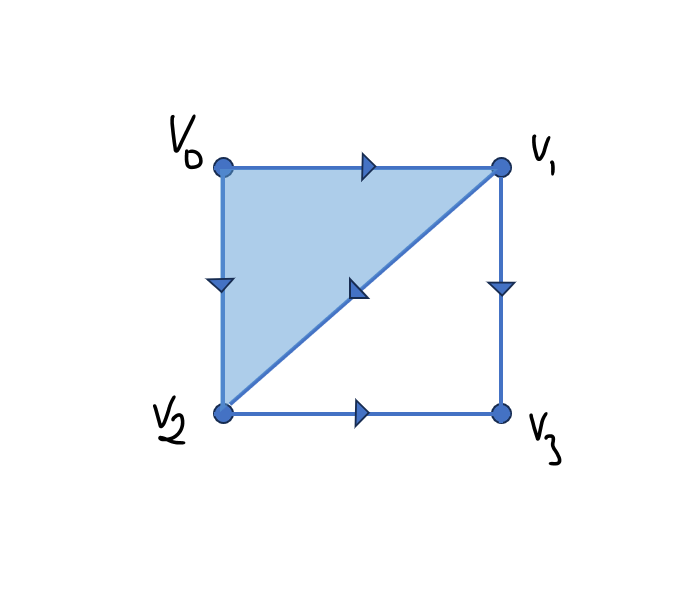
\includegraphics[width = 8cm, height = 6cm]{SimplicialComplexexample1.png}
    \caption{Geometric realization of the simplicial complex X defined as above.}
    \label{SCExample 1}
\end{figure}
\begin{example} Torus $\mathbb{T}^2$
\end{example}
\begin{figure}[h!]
    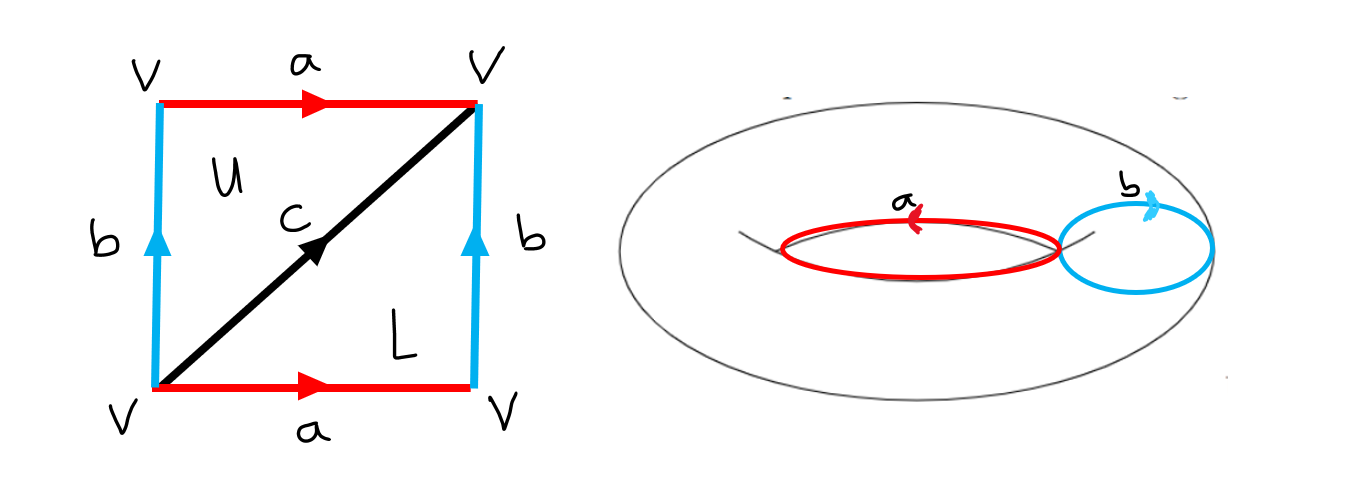
\includegraphics[width = 16cm, height = 6cm]{Complex structure torus.png}
    \caption{The $\Delta$-complex struture for a torus $\mathbb{T}^2$}
    \label{fig:delta-complex structure torus}
\end{figure}

\begin{itemize}
    \item $[v]$ = v : $\Delta^0 \rightarrow X$
    \item $[v,v]$ = a : $\Delta^1 \rightarrow X$
    \item $[v,v]$ = b : $\Delta^1 \rightarrow X$
    \item $[v,v]$ = c : $\Delta^1 \rightarrow X$
    \item $[v,v,v]$ = U : $\Delta^2 \rightarrow X$
    \item $[v,v,v]$ = L : $\Delta^2 \rightarrow X$
\end{itemize}

\subsection{Simplicial homology}
The goal for this section is to define the simplicial homology groups of a simplicial complex $X = (V, \Sigma)$. Homology theory in algebraic topology comes in many different types; but all satisfy a set of axioms. Homology is a functor on an abelian category; associates a topological space $X$ to a sequence of abelian algebras such as groups or $R$-modules. We will shine light to simplicial homology a variant of homology that computes algebraic structures to provide a mathematical way of quantifying invariants: the holes, voids, and higher dimensional equivalences of the topological space X. Homology translates a topological problem into an algebraic problem unlocking the use of algebraic objects to quantify the homology groups and compute algebraic invariants to distinguish spaces. 
Simplicial homology groups involve understanding how cycles and boundaries of n-simplices relate to each other. The first homology group,$H_1(X)$, conveys information on the one-dimensional holes or loops in the space, while the second homology group, $H_2(X)$ captures the two-dimensional voids or cavities. Each homology group corresponds to a different dimension of the topological features, providing a concise summary of the shape of space X.

%For TDA, simplicial homology groups have invaluable applications. They help identify persistent features in datasets and quantify essential topological characteristics.\\
As mentioned above simplicial homology is a functor. In general, a functor in category theory is a mapping between categories where a category is a collection of 'objects' linked by 'morphisms'. 

\begin{definition} Let $\mathcal{C}$ and $\mathcal{D}$ be categories. A functor $\textbf{F}$ from $\mathcal{C}$ to $\mathcal{D}$ maps,
\begin{itemize}
    \item each object $X \in \mathcal{C}$ to an object $F(X) \ in \mathcal{D}$,
    \item each morphism $f: X \to Y$, $f \in \mathcal{C}$ to a morphism $F(f): F(X) \to F(Y)$, $F(f) \in \mathcal{D}$ such that the two following condition are satified:
    \begin{itemize}
        \item $F(id_{X}) = id_{F(X)}$ for every object $X \in \mathcal{C}$,
        \item $F(f \circ g) = F(g) \circ F(g)$ for all morphisms $f:X \to Y$ and $g:Y \to Z$, $f,g \in \mathcal{C}$
    \end{itemize}
\end{itemize}
\end{definition}
Simplicial homology functor can be thought as a two part functor. The first functor maps the category of topological spaces, $\textbf{Top}$, to chain complexes $\textbf{Comp}$. The second functor then maps the chain complexes to abelian algebras $\textbf{Ab}$. The first category of focus will be the category of chain complexes with chain complexes as objects and chain maps as morphisms. The construction of simplicial complexes in the previous subchapter will be used to define simplicial chain complexes which then leads to the introduction and definition of homology groups and its functorality.  
In this paper, we will stick to the generalisation and use $R$ to denote a commutative ring with unity to then define $R$-modules abelian algebras.
Let's now apply the notion of $R$-modules to simplicial complexes to turn our combinatorial geometric object into an algebraic object.
\begin{definition}
A \textbf{simplicial k-chain} is a finite collection or sum of all $k$-simplices in the oriented simplicial complex X,
\be
\sum_\alpha n_\alpha \sigma_\alpha ,
\ee
where coefficients $n_\alpha \in R$, $k$-simplex $\sigma_\alpha = [v_0,...,v_k] \in X$, and $\alpha$ is the indexing set.
\end{definition}
For a simplicial complex X, denote $C_k(X,R)$ the free R-module generated by the $k$-simplices of X,
\be
C_k(X,R) = \{\Sigma_\alpha n_\alpha \sigma_\alpha | n_\alpha \in R, \sigma_\alpha \in X\}
\ee
If R is a field $k$ = $\mathbb{Q}, \mathbb{R}, \mathbb{C}, or \mathbb{Z_p}$ for $p$ prime then $C_k(X,R)$ is a $k$-vector space. If R = $\mathbb{Z}$, then $C_k(x,R)$ is a $\mathbb{Z}$-module which is a free abelian group. We aim to construct an algebraic structure from the simplicial complex by forming a sequence of $C_k(X,R)$ with a boundary homomorphism defined as follows:
\begin{definition}
    The \textbf{boundary homomorphism} is a map
\be
\partial_k : C_k(X,R) \rightarrow C_{k-1}(X,R),
\ee
defined as
\be
\partial_k(\sigma_\alpha) = \Sigma_i (-1)^i [v_0,...,\hat{v}_i,...,v_k],
\ee
\end{definition} where $\hat{v_i}$ denotes the omitted vertex and $k$-simplex $\sigma_\alpha = [v_0,...,v_k] \in X$ .

The boundary operator on a general $k$-simplex is the sum of $(k-1)$-simplices.
\begin{example}
Returning back to the previous example. Let X be a simplicial complex having a vertex set $V =\{v_0, v_1, v_2, v_3\}$ with a choice of order $v_0 < v_1 < v_2 < v_3$. X has 4 0-simplices $[v_0], [v_1], [v_2], [v_3]$,5 1-simplices $[v_0,v_1],[v_0,v_2],[v_1,v_2],[v_1,v_3]$ and $[v_2,v_3]$ and a 2-simplex $[v_0, v_1, v_2]$. Applying the boundary operator we obtain:\\
The geometric realisation for a 0-simplex is a vertex. One can see quite clearly that a vertex does not have a boundary and so the boundary operator $\partial_0$ on each of the 0-simplices is the zero map.\\
$\partial_0[v_0] = \partial_0[v_1]= \partial_0[v_2]= \partial_0[v_3] = 0$ \\
$\partial_1[v_0,v_1] = [v_1] - [v_0],$\\
$\partial_1[v_0,v_2] = [v_2]- [v_0],$ \\
$\partial_1[v_1,v_2] = [v_2] - [v_1],$\\
$\partial_1[v_1,v_3] = [v_3] - [v_1],$\\
$\partial_1[v_2,v_3] = [v_3]- [v_2], $ \\
$\partial_2[v_0,v_1,v_2] = [v_1,v_2] - [v_0,v_2] + [v_0,v_1]$
\end{example}
Together, simplicial chains and the boundary R-homomorphisms form a sequence of $R$-modules $C_k(X,R)$ called a chain complex.
\begin{definition} A \textbf{chain complex }$\mathcal{C}_{*} = (C_{k})^{\infty}_{k=0}$ of X, is a sequence of chain complexes and boundary R-homomorphisms
\be
...\rightarrow C_{k+1}(X,R) \xrightarrow{\partial_{k+1}} C_k(X,R)\xrightarrow{\partial_k}...\rightarrow C_1(X,R)\xrightarrow{\partial_1}C_0(X,R)\xrightarrow{\partial_0} 0
\ee
such that $\partial_k o \partial_{k+1} = 0$ for all k.
\end{definition}
%Using the $\Delta$-complex structure of the torus $\mathbb{T}^2$ as an example to apply the boundary homomorphism.\\
%As the boundary homomorphism maps chains of higher dimensions to lower dimensions, the $\partial_{3}$ and $\partial_0$ are the zero maps. 
%\be
%\partial_0(\Delta_0(\mathbb{T}^2))= 0
%\ee
%\be
%\partial_1(\Delta_1(\mathbb{T}^2))= \partial(a) + \partial(b) + \partial(c) = (v-v) + (v-v) + (v-v) = 0
%\ee
%\be
%\partial_2(\Delta_2(\mathbb{T}^2)) = \partial(pU) + \partial(qL) = (p+q)(a+b-c) = 0 \iff p=-q
%\ee

The simplicial homology groups themselves are algebraic in nature, representing the quotient of equivalence classes of cycles and boundaries of the simplicial complex. A cycle is a combination of simplices (chains) that forms a closed loop or higher-dimensional analogs with no "boundary." Define the group of cycles as the kernel (nullspace) of the boundary R-homomorphism
\begin{definition}The $\textbf{k-dimensional cycle group}$ is defined as the kernel of the homomorphism $\partial_{k}$,
\be
Z_k = ker(\partial_k) = \{c \in C_k(X,R)|  \partial_k(c) = 0 \}.
\ee
\end{definition}
On the other hand, a boundary of a $k+1$-simplex can be expressed as a combination of $k$-simplices
\begin{definition}
The $\textbf{k-dimensional boundary group}$ is defined as the image of the operator $\partial_{k+1}$,
\be
B_k = im(\partial_{k+1}) = \{d \in C_k(X,R) | \exists c \in C_{k+1} : d = \partial_{k+1}(c)\}
\ee
\end{definition}
$Z_k$ and $B_k$ together with the addition operator form subgroups of $C_k(X,R)$.\\
An implication of $\partial_k\partial_{k+1} = 0$ is that $im(\partial_{k+1}) \subset ker(\partial_k)$. \\
\textit{Proof}:\\
Let $\alpha \in C_{k+1}$ be a simplicial chain. Then, $\partial_{k+1}(\alpha) \in im(\partial_{k+1})$. If $\alpha$ a cycle then $\partial_{k+1}(\alpha) = 0$ and so $\partial_{k+1}(\alpha) \in im(\partial_{k+1}) \subset ker(\partial_k)$. If $\alpha$ is not a cycle then $\alpha$ has boundary. By the definition of a chain complex, $\partial_{k} \circ \partial_{k+1}(\alpha) = 0$ and so $\partial_{k+1}(\alpha) \in im(\partial_{k+1}) \subset ker(\partial_{k})$.

Therefore, we define the $kth$-homology group $H_k$ as the quotient group of $Z_k$ and $B_k$,
\begin{definition}
The $\textbf{kth-homology group}$ of a chain complex $\mathcal{C_{*}}$ is,
\be
H_k(X,R) = \frac{Z_k}{B_k}
\ee
\end{definition}

Using group theory knowledge, the rank of a group is the size of the basis (minimal generating set).
\begin{example} Returning, again, to our simplicial complex X. We have calculated the boundary operator on its $k$-simplices:\\
$\partial_0[v_0] = \partial_0[v_1]= \partial_0[v_2]= \partial_0[v_3] = 0$ \\
$\partial_1[v_0,v_1] = [v_1] - [v_0],$\\
$\partial_1[v_0,v_2] = [v_2]- [v_0],$ \\
$\partial_1[v_1,v_2] = [v_2] - [v_1],$\\
$\partial_1[v_1,v_3] = [v_3] - [v_1],$\\
$\partial_1[v_2,v_3] = [v_3]- [v_2], $ \\
$\partial_2[v_0,v_1,v_2] = [v_1,v_2] - [v_0,v_2] + [v_0,v_1]$\\
Let's calculate the $H_0$ homology group. By choosing $v_1-v_0, v_2 - v_0, v_3 - v_2,$ and $v_0$ as a basis for $Z_0$ and $v_1-v_0, v_2 - v_0, v_3 - v_2$ as a basis for $B_0$ we have that,\\
\be
H_0 = \frac{Z_0}{B_0} = \frac{ker(\partial_0)}{im(\partial_1)} = R
\ee with the vertex $v_0$ as the generator.
Similarly, for $H_1$, $Z_1$ is generated by $[v_1,v_2] - [v_0,v_2] + [v_0,v_1]$ and $[v_2,v_3] - [v_1,v_3] + [v_1,v_2]$ and $B_1$ is generated by $[v_1,v_2] - [v_0,v_2] + [v_0,v_1]$ and so,
\be
H_1 = \frac{Z_1}{B_1} = R
\ee
Lastly, for $H_2$, since $\partial_2[v_0,v_1,v_2] = [v_1,v_2] - [v_0,v_2] + [v_0,v_1]$ we see that $\partial_2$ is injective and so $Z_2 = \partial_2$ = 0,
\be
H_2 = \frac{Z_2}{B_2}= 0
\ee
\end{example}
\begin{definition}
The $\textbf{nth Betti number}$, $\beta_n$, of X is the rank of the $n$th homology group of a chain complex $\mathcal{C_{*}}$ is,
\be
\beta_n = rank(H_n) = rank(Z_n) - rank(B_n).
\ee
\end{definition}

For each dimension $n \in \mathbb{Z}$, there is a Betti number which corresponds to the size of the basis for homology group in that dimension.  For $0$-simplices, $\beta_0$ is the number of connected components of X. For $1$-simplices, $\beta_1$ is the number of non-contractible closed loops or holes in X. For $2$-simplices, $\beta_2$ is the number of non-contractible closed surfaces in X.
\begin{definition} A \textbf{simplicial map} from X to Y, where X and Y are two simplicial complexes, is a function that maps the vertex set of X to the vertex set of Y, $f: V_x \to V_y$ , and maps every simplex in X to a simplex in Y, for any $\sigma \in X, f(\sigma) \in Y$.
\end{definition}
\begin{definition} Let $(\mathcal{C}_{*}, \partial)$ be the chain complex of a topological space $X$ and $(\mathcal{D}_{*},\overline{\partial})$ be the chain complex of a topological space $Y$. Then a \textbf{chain map} between the chain complexes is a collection of maps $f = \{f_k: C_k \to D_k\}$ such that
\be
f_{k-1}\circ \partial = \overline{\partial}\circ f_{k}
\ee
\end{definition}
and the following diagram commutes\\

\begin{tikzpicture}[>=triangle 60]
  \matrix[matrix of math nodes,column sep={60pt,between origins},row
    sep={60pt,between origins},nodes={asymmetrical rectangle}] (s)
  {
     &|[name=c0]| ... &|[name=c1]| C_{k+1} &|[name=c2]| C_{k} &|[name=c3]| C_{k-1} &|[name=c4]| ... \\
    %
     &|[name=d0]| ... &|[name=d1]| D_{k+1} &|[name=d2]| D_{k} &|[name=d3]| D_{k-1} &|[name=d4]| ... \\
  };
  \draw[->] 
            (c1) edge node[auto] {\($f_{k+1}$\)} (d1)
            (c2) edge node[auto] {\($f_{k}$\)} (d2)
            (c3) edge node[auto] {\($f_{k-1}$\)} (d3)
            (c0) edge node[auto] {\($\partial_{k+2}$\)} (c1)
            (c1) edge node[auto] {\($\partial_{k+1}$\)} (c2)
            (c2) edge node[auto] {\($\partial_k$\)} (c3)
            (c3) edge node[auto] {\($\partial_{k-2}$\)}(c4)
            (d0) edge node[auto] {\($\overline{\partial}_{k+2}$\)}(d1)
            (d1) edge node[auto] {\($\overline{\partial}_{k+1}$\)}(d2)
            (d2) edge node[auto] {\($\overline{\partial}_k$\)} (d3)
            (d3) edge node[auto] {\($\overline{\partial}_{k-2}$\)}(d4)
  ;
\end{tikzpicture}
\\
Simplicial Homology is a functor that assigns R-module chain complexes to abelian R-modules and R-homomorphisms to R-homomorphisms. The functoriality property of homology on the chain complexes above induces R-homomorphisms between the homology of the two complexes

\begin{proposition}\label{chain map induced homo} A chain map between chain complexes induces R-homomorphisms between the homology of two complexes
\end{proposition}
For a chain map $f = \{f_k: C_k \to D_k\}$ , the induced homomorphism 
\be
f_{*}: H_{k}(X,R) \to H_{k}(Y,R)
\ee
is defined as $f_{*} (\sigma) = f \circ \sigma$ where $\sigma$ is a $k$-simplex of $X$. We can extend the definition of $f_{*}$ (R)-linearly and obtain,
\be
f_{*}(\Sigma_\alpha n_\alpha \sigma_\alpha) = \Sigma_\alpha n_\alpha f_{*}(\sigma_\alpha)
\ee
such that,
\be
f_{*}\partial = \overline{\partial}f_{*}.
\ee\\
\textit{Proof}:
Since Homology is defined by the cycle groups and boundary groups, it suffices to check that the chain map $f = \{f_k: C_k \to D_k\}$ maps cycles to cycles and boundaries to boundaries between the chain complexes $\mathcal{C}$ and $\mathcal{D}$.
\begin{itemize}
    \item f maps cycles to cycles: Let $\alpha \in C_n$ such that $\partial(\alpha) = 0$. Then,
    \be
    \overline{\partial}f(\alpha) = f\partial(\alpha) = f(0) = 0.
    \ee and so $f(\alpha) \in D_{k+1}$ is a cycle.

    \item f maps boundaries to boundaries: Let $\beta \in C_n$. Then,
    \be
    f\partial(\beta) = \overline{\partial}f(\beta),
    \ee
\end{itemize}
Hence f induces an R-homomorphism $f_{*}: H_{k}(X,R) \to H_{k}(Y,R)$. This notion of induced R-homomorphisms between chain complexes will be important in defining persistent homology the main tool for TDA. 


\begin{proposition}The induced map of the composition is the composition of the induced maps. Let $f: X \to Y$ and $g:Y\to Z$ be continuous chain maps then,
\be
(g \circ f)_{*} = g_{*} \circ f_{*}
\ee
Additionally,
\be
(Id_{X})_{*} = Id_{H_{*}(X)}
\ee
\end{proposition}
\textit{Proof}: By definition of induced chain map,
\be
(g \circ f)_{*}(\sigma) = (g \circ f) \circ \sigma = g \circ (f \circ \sigma) = g \circ f_{*}(\sigma) = g_{*} \circ f_{*}(\sigma)
\ee and,
\be
(Id_{X})_{*}(\sigma) = Id_{X} \circ \sigma = \sigma
\ee


\begin{definition}Let X and Y be two toplogical spaces and let $f:X\to Y$ and $g:X\to Y$ be two continuous maps. The maps $f$ and $g$ are \textbf{homotopic} if there exists a continuous map
\be
H: X \times I \to Y
\ee such that for all $x \in X$ we have that,
\be
H(x,0) = f(x),
\ee and
\be
H(x,1) = g(x).
\ee
\end{definition}

\begin{proposition}\label{homotopic maps induced} Let $f:X\to Y$ and $g:X\to Y$ be two continuous maps between topological spaces $X$ and $Y$. If $f$ and $g$ are homotopic $f \simeq g$ then they induce the same $R$-homomorphism at the level of homology,
\be
f_{*} = g_{*}: H_{k}(X,R) \to H_{k}(Y,R).
\ee
\end{proposition}


\begin{definition} Let X and Y be two topological spaces and let $f: X \to Y$ and $g: Y \to X$  be a continuous maps. X and Y are said to be homotopy equivalent $X \simeq Y$ if,
\be
f \circ g \simeq id_{Y},
\ee and
\be
g \circ f \simeq id_{X}
\ee
\end{definition}
f and g are called homotopy equivalences. The following proposition will be important when constructing \v{C}ech complexes for computing persistent homology. We will see that the 'thickening' of the dataset via metric balls around each point is the 'same' as the original discrete dataset. The dataset can be deformed into to this 'thickening'. Two such spaces are called homotopy equivalent. The proposition below will be of importance when Nerve theorem and \v{C}ech complexes are introduced.
\begin{proposition}\label{induced homotopy equivalence} The maps $f_{*}: H_{k}(X,R) \to H_{k}(Y,R)$ induced by a homotopy equivalence $f:X \to Y$ are isomorphisms for all k.
\end{proposition}
\textit{Proof}:\\ Since $X$ and $Y$ are homotopy equivalent there are continuous maps $f:X \to Y$ and $g:Y \to X$ such that 
\be
f \circ g \simeq id_{Y},
\ee and
\be
g \circ f \simeq id_{X}
\ee by Prop.\ref{homotopic maps induced} we have strict equality bewtween the induced maps of the homotopic maps,
\be
(f \circ g)_{*} = f_{*} \circ g_{*} = (id_Y)_{*} = id_{H_{*}(Y)},
\ee
\be
(g \circ f)_{*} = g_{*} \circ f_{*} = (id_X)_{*} = id_{H_{*}(X)}.
\ee
imply that $f_{*}$ and $g_{*}$ are inverses of each other and so $f_{*}$ and $g_{*}$ are isomorphisms for all k.


\section{Simplicial Complex Construction of a Dataset}
Obtaining the simplicial complex structure is the first and essential step to calculate the homology groups of the space.The simplicial complex of a topological space that is know is easy to construct and compute with. However, datasets that involve high dimensional points and a large number of data points, the underlying simplicial complex becomes a challenge to understand the topological space the points lie on. How could one build a simplicial complex from a dataset without any prior knowledge of the structure and topological properties? Assume that the dataset is in the form of a discrete finite point cloud
\be
\mathbb{X} \subset \mathbb{R}^n
\ee
Currently, there are only $0$-simplices (vertices) in the point cloud and this provides ineffectual information about the underlying topological space (except for the number of points). Data scientists and computer scientist who may be reading this paper might be familar with a machine learning classification algorithm called K-Nearest Neightbour. Essentially to construct the simplicial complex an analogous method will be applied. Take a distance paramter $\epsilon $ and vary its value. As the value varies, obtain an open cover $U = B(x_i,\epsilon)$ defined by open balls around $x_i$ where $x_i \in \mathbb{X}$ are the data points. Include higher dimensional $k$-simplices to the simplicial complex if the open balls intersect and define a sequence of filtration of simplicial complexes with the inclusion maps as chain maps between the evolving complex $C^{\epsilon}$. Together the filtration, the inclusion maps and the boundary maps between the decreasing dimension of chain complexes form a gigantic lattice family of chain complexes called a persistent complex. After this construction, the homology techniques developed in the previous chapter can be applied to compute the lifespan of the homological features (connected components, loops, voids and higher dimensional equivalences) and to visualised through barcode graphs and persistent diagrams.
In the literature, you may encounter many different types of complexes. The most common complexes used in practice are \v{C}ech and Vietoris-Rips and so in this paper we will focus on the two. 
We begin with the assumption that our discrete finite point cloud $\mathbb{X}$ is a subset of $\mathbb{R}^n$ where $\mathbb{R}^n$ is endowed with a metric $d$. Hence, we have a metric space $(\mathbb{R},d)$.
\begin{definition}If $(X,d)$ is a metric space and $Y \subseteq X$ we can define \be
d_Y : Y \times Y \to \mathbb{R},
\ee
to be the \textbf{induced metric} of $d: X \times X \to \mathbb{R}$. That is,
\be
d_Y(a,b) = d(a,b) 
\ee
for all $a,b \in Y$.
\end{definition}

\begin{definition} Given a metric space $(X,d)$ for $x \in X$ and $\epsilon>0$, define $B_{\epsilon}(x) = \{y \in X : d(x,y) < \epsilon\}$ to be the ball of radius $r$ centered at $x$. The collection of all balls $B_{\epsilon}(x)$ for $x \in X$ and $\epsilon>0$ is a basis for the metric topology on $X$ induced by $d$.
\end{definition}

\begin{definition} An \textbf{$\epsilon$-thickening} of a metric space $X$ is a larger metric space $X \subseteq Z$ such that,
\begin{itemize}
    \item the metric d on $Z$ extends that on $X$,
    \item $d(z,X) \leq \epsilon$ for all $z \in Z$
\end{itemize}
\end{definition}
In terms of metric toplogy, $\epsilon$-thickening is the union of $B_{\epsilon}(x)$ for all $x \in X$. 

\subsection{Vietoris-Rips and \v{C}ech Complexes}

\begin{definition} Given a point cloud $\mathbb{X} \subset \mathbb{R}^n$ and $\epsilon > 0$, the \textbf{Vietoris-Rips complex} $VR_{\epsilon}(\mathbb{X})$ is the abstract simplicial complex whose vertex set is the set of points of $x_i \in \mathbb{X}$, and whose $k$-simplices are given by all $k+1$ vertices ${x_0, ..., x_k}$ that are pairwise less than $\epsilon$ apart. That is, a simplex  $\sigma = [x_0, ..., x_k]$ is in $VR_{\epsilon}(\mathbb{X})$ if
\be
x_j \in B_{\epsilon}(x_i) 
\ee
for all $0 \leq i,j \leq k$. 

\be
VR_{\epsilon}(\mathbb{X}) = \{\sigma = [x_0,...,x_k] : x_j \in B_{\epsilon}(x_i)  \forall  0 \leq i,j \leq k \}
\ee
\end{definition}
Vietoris-Rips complex can be thought of as the $\epsilon$-thickening of the given point cloud $\mathbb{X}$ with the inclusion of $k$-simplices of neighboring $k+1$ vertices satisfying the distance parameter. 

\begin{definition}Let $X$ be a topological space. A non-empty and finite collection of subsets $\mathcal{U} = \{U_i : i \in I\}$ where $U_i \subset X$ is called a \textbf{cover} of $X$ if $X \subseteq \bigcup_{i\in I} U_{i}$.
\end{definition}

\begin{definition}Given a cover of a topological space X, $\mathcal{U}$, as defined as above. The \textbf{nerve} of the cover is the abstract simplicial complex $\mathcal{N}(\mathcal{U})$ whose $k$-simplicies are determined by $k+1$ elements of $\mathcal{U}$ that have non-empty intersection. That is,
\be
\sigma = [U_{i_0}, .., U_{i_k}] \in \mathcal{N}(\mathcal{U}) \iff \bigcap^{k}_{n=0} U_{i_n} \neq \emptyset
\ee
\end{definition}

\begin{theorem}\textbf{(Nerve Theorem)} Let $\mathcal{U} = \{U_i : i \in I\}$ be a cover of a topological space X such that for any $I' \subseteq I$, the intersection $\bigcap_{i\in I'}U_i$ is either empty or contractible. Then, X and the nerve $\mathcal{N}(\mathcal{U}$) are homotopy equivalent.
\end{theorem}


\begin{definition} The \textbf{\v{C}ech Complex} of radius $\epsilon > 0$ on the point cloud $\mathbb{X} \subseteq \mathbb{R}^n$ is the abstract simplicial complex defined as,
\be
\v{C}ech_{\epsilon}(\mathbb{X}) = \{\sigma = [x_o,...,x_k] : \bigcap^{k}_{i=0} \overline{B(x_i, \epsilon)}\neq \emptyset, x_i \in \mathbb{X}\}
\ee
whose $k$- simplices are given by $k+1$ vertices $\sigma = [x_o,...,x_k]$. 
\end{definition}
The \v{C}ech complex of a point cloud $\mathbb{X}$ for a given value of $\epsilon >0$ is the nerve of the covering of $\mathbb{X}$ by closed balls.As the intersection of closed balls in the metric space $\mathbb{R}^n$ is convex and so the intersection is contractible. Hence, it follows from the Nerve Theorem that the \v{C}ech complex is homotopy equivalent to the $\epsilon$-thickening and hence homotopy equivalent to the point cloud $\mathbb{X}$. By Prop.\ref{induced homotopy equivalence} the homotopy equivalence map $f: \mathbb{X} \to \v{C}ech_{\epsilon}(\mathbb{X})$ induces isomorphisms between their $kth$-homology groups. So to observe homology of the point cloud set $\mathbb{X}$ it suffice to observe the homology of the \v{C}ech complex $\v{C}ech_{\epsilon}(\mathbb{X})$.

Both the \v{C}ech and Vietoris-Rips complex involve the use of the $\epsilon$-thickening of the point cloud. 
There is a relationship between these two simplicial complexes and it is given in the following propostition,
\begin{proposition} For any given point cloud $\mathbb{X}$ and $\epsilon > 0 $,
\be
VR_{\epsilon}(\mathbb{X}) \subseteq \v{C}ech_{\epsilon}(\mathbb{X}) \subseteq VR_{2\epsilon}(\mathbb{X}).
\ee
\end{proposition}


The \v{C}ech complex is bounded above and below by the Vietoris-Rips complexes of parameters $2\epsilon$ and $\epsilon$ respectively. In the construction of the \v{C}ech complex, one has to keep track of intersections of the closed balls. The number of intersections can be very large as the number of data points in the point cloud increases and so computing with the \v{C}ech complex is computationally expensive. Hence, it suffices to use the Vietoris-Rips complex for computations.\\

Now the question arises, what value of $\epsilon$ is the best to reveal the underlying structure? The unfortunate answer is that there is none. Instead, consider a sequence of nested simplicial subcomplexes of $\mathbb{X}$. This sequence is known as a filtered simplicial complex.\\

Given a point cloud $\mathbb{X}$, construct the simplicial complex of your choice. In this case, we will use the Vietoris-Rips complex,
\be
VR_{\epsilon}(\mathbb{X}) = \{\sigma = [x_0,...,x_k] : x_j \in B_{\epsilon}(x_i)  \forall  0 \leq i,j \leq k \}
\ee

Shown schematically in Fig.\ref{fig:Filtration}, as the value of $\epsilon$ increases the open balls around each point increases.

\begin{figure}[h]
    \centering
    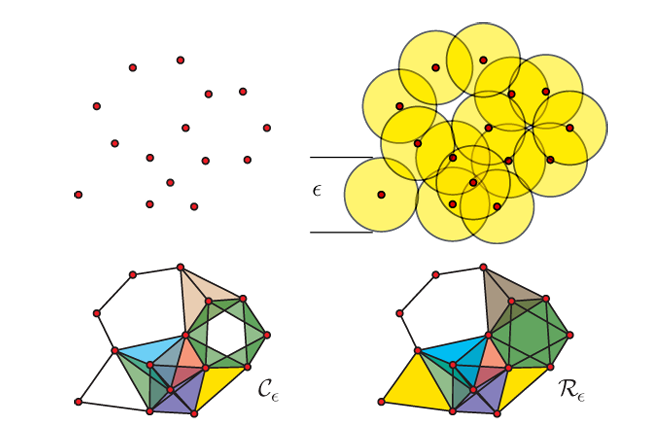
\includegraphics{cech and rips robert ghrist.png}
    \caption{Schematic diagram for the filtration process of obtaining the filtered simplicial complex \cite{Ghrist2007BarcodesTP}}
    \label{fig:Filtration}
\end{figure}
For ease of notation, denote the Vietoris-Rips complex of $\mathbb{X}$ with distance parameter $\epsilon$ by 
\be
\mathbb{X}_{\epsilon} = VR_{\epsilon}(\mathbb{X}).
\ee

\begin{definition}A filtration of a simplicial complex X is a nested family of subcomplexes $(X_{i})_{i \in I}$ where $I \subseteq \mathbb{R}$ such that if $i,j \in I$ and $i \leq j$ then $X_{i} \subseteq X_{j}$ and $X = \bigcup_{i\in I} X_{i}$.
\end{definition}
The filtered complex sequence of the point cloud $\mathbb{X}$ is an ascending sequence of simplicial subcomplexes,
\be
\emptyset \subseteq \mathbb{X}_{\epsilon_0} \subseteq \mathbb{X}_{\epsilon_1} \subseteq ... \subseteq \mathbb{X}_{\epsilon_{max}} = \mathbb{X}.
\ee
Since the Vietoris-Rips complex is a simplicial complex, the filtration forms a chain complex with the inclusion maps $\iota_{(i,j)}: \mathbb{X}_{i} \to \mathbb{X}_{j} $ for $i\leq j$ as the chain maps. By Prop.\ref{chain map induced homo} these chain maps induces R-homomorphisms between the homology groups.



\section{Persistent homology}
Persistent homology is one of the main techniques used in TDA \cite{akingbade2023topological}\cite{ravishanker2019topological}\cite{AZComputePH}\cite{CarlssonTDAappli}. By using one of the methods introduced above; if one computes the homology group of a single value of $\epsilon$ it will only provide a "snapshot" of the topological story and convey very little information of the underlying shape of the space on which the data lies on\cite{CarlssonTDAappli}.Persistent homology quantifies the notion of the persistence of topological features of a space and hence provides a method to track these properties and identity the dominant features. We will start this section with some definitions and notions of the mathematical structure of persistent homology, then provide two graphical interpretations of persistence. 
\begin{definition}
A \textbf{persistence complex} $\mathfrak(C)$ is a family of chain complexes $\{C^{i}_{*}\}_{i\geq 0}$ over R, together with chain maps $f^{i} : C^{i}_{*} \rightarrow C^{i+1}_{*}$ between chain complexes.
\end{definition}


\begin{tikzpicture}[>=triangle 60]
  \matrix[matrix of math nodes,column sep={60pt,between origins},row
    sep={60pt,between origins},nodes={asymmetrical rectangle}] (s)
  {
    &|[name=c30]|  &|[name=c31]|   &|[name=c32]|  \\
    %
    &|[name=c20]| C^{0}_{2} &|[name=c21]| C^{1}_{2} &|[name=c22]| C^{2}_{2} &|[name=02]| ... \\
    %
    &|[name=c10]| C^{0}_{1} &|[name=c11]| C^{1}_{1} &|[name=c12]| C^{2}_{1} &|[name=01]| ... \\
    %
    &|[name=c00]| C^{0}_{0} &|[name=c01]| C^{1}_{0} &|[name=c02]| C^{2}_{0} &| [name= 00]| ...\\
    %
    &|[name = a]| 0 & | [name = b] | 0 &| [name = c] | 0 \\
  };
  \draw[->] (c30) edge node[auto] {\($\partial_3$\)} (c20)
            (c31) edge node[auto] {\($\partial_3$\)} (c21)
            (c32) edge node[auto] {\($\partial_3$\)} (c22)
            (c20) edge node[auto] {\($\partial_2$\)} (c10)
            (c21) edge node[auto] {\($\partial_2$\)} (c11)
            (c22) edge node[auto] {\($\partial_2$\)} (c12)
            (c10) edge node[auto] {\($\partial_1$\)} (c00)
            (c11) edge node[auto] {\($\partial_1$\)} (c01)
            (c12) edge node[auto] {\($\partial_1$\)} (c02)
            (c00) edge node[auto] {\($\partial_0$\)} (a)
            (c01) edge node[auto] {\($\partial_0$\)} (b)
            (c02) edge node[auto] {\($\partial_0$\)} (c)
            (c20) edge node[auto] {\($f^{0}$\)} (c21)
            (c21) edge node[auto] {\($f^{1}$\)} (c22)
            (c22) edge node[auto] {\($f^{2}$\)} (02)
            (c10) edge node[auto] {\($f^{0}$\)} (c11)
            (c11) edge node[auto] {\($f^{1}$\)} (c12)
            (c12) edge node[auto] {\($f^{2}$\)} (01)
            (c00) edge node[auto] {\($f^{0}$\)} (c01)
            (c01) edge node[auto] {\($f^{1}$\)} (c02)
            (c02) edge node[auto] {\($f^{2}$\)} (00)
  ;
\end{tikzpicture}
\\
The above diagram displays a section of the persistence complex. The dimensions of the complexes decreases vertically to the bottom under the boundary homomorphism $\partial_n$. While the filtration index increases to the right under the chain maps $f^{i}$. Chain maps between chain complexes induces homomorphisms between the homology groups of the two complexes.

\begin{definition}
A \textbf{persistence module} $M$ is a family of $R-$modules $M^{i}$, together with $R$-homomorphisms $\phi^{i} : M^{i} \rightarrow M^{i+1}$.
\end{definition}


The application of the homology functor on the persistence chain complex induces a chain of $R-$ modules. The homology of the persistence chain complex produces a persistence module. The chain maps $f^{i} : C^{i}_{*} \rightarrow C^{i+1}_{*}$ induces homomorphisms on the homology groups $H_n(C^{i}_{*}, R)$. This homology $H_n(C^{i}_{*}, R)$ preserves the $R$-module structure but is not necessary free \cite{Ghrist2007BarcodesTP}.\\

It was developed by Carlsson and Zomorodian \cite{AZComputePH} that a finite persistence module has the structure of a graded module over $k[x]$, where $k$ is a field, since graded ideals of $k[x]$ are of the form $<x^i>$ \cite{HSchenckAlgebraicFound}\cite{AZComputePH}.
The filtered simplicial complex with inclusion maps produces an persistence chain complex \cite{CarlssonAMS}\cite{AZComputePH}. In the section on simplicial complex, the chain complex was a chain of free abelian groups or $\mathbb{Z}$-modules. For a persistence chain complex, fix a principal ideal domain (PID) of coeffcients R and place a graded $R[x]$-module structure on the filtered simplicial complex. This allows it to be free as an $R[x]$-module.


\begin{definition}
For $i < j$, the \textbf{(i,j)-persistent homology} $H^{i\rightarrow j}_{*} (C^{i}_{*}) $ of $C^{i}_{*}$ is defined to be the image of the induced homomorphism $\phi^{i} : H^{i}_{*} (C^{i}_{*}) \rightarrow H^{j}_{*} (C^{i}_{*})$ 
\end{definition}

The two following theorems are from Carlsson and Zomorodian "Computing Persistent Homology" \cite{AZComputePH} and Ghrist "Barcodes:The persistent topology of data" \cite{Ghrist2007BarcodesTP}.
\begin{theorem}
\textbf{Structure Theorem}:For a finite persistence module $H_n(C^{i}_{*}, k)$ with field $k$ coefficients,
\be\label{StuctureTheorem}
H_n(C^{i}_{*}, k) \cong \bigoplus_{i} x^{t_i} k[x]\oplus \Biggl(\bigoplus_{j} x^{r_{j}} (k[x]/ (x^{s_j}k[x]))\Biggr),
\ee
for some $t_{i}, r_{j},s_{j} \in \mathbb{Z}_{\geq 0}$.
\end{theorem}

The \textit{free component}, $x^{t_i} k[x]$, includes generators of the homology groups and may generate an infinite number of elements. It is a vector space of dimension $t_{i}$.The \textit{torsional component}, $\bigoplus_{j} x^{r_{j}} (k[x]/ (x^{s_j}k[x]))$ includes generators of the homology groups that may generate a finite number of elements that "appear at parameter $r_{j}$ and disappear at parameter $r_{j} + s_{j}$" \cite{Ghrist2007BarcodesTP}. These appearances and disappearances of generators correspond to the births and deaths of generators of $C^{i}_{*}$. This theorem leads to the characterisation of barcodes.
\subsection{Barcodes and Persistent diagrams}\label{BARCODES}
The topological information computed by persistent homology can be displayed using persistent diagrams or barcode diagrams showing 'birth', 'persistence', and 'death' of intrinsic features of the topological space built from the filtered simplical complex homology. Both convey the same information in slightly different ways. Barcodes highlights the homology classes through bars where it appears at time $t = b_i$ (birth) until it merges with a different connected component an disappears at time $t=d_i$ (death) for $i \in I$. Whereas persistence diagram visualises each bar as a point with coordinates $(b_i,d_i)_{i \in I}$.
\begin{theorem}
    The rank of the persistent homology group $H^{i\rightarrow j}_n(C^{i}_{*}, k)$ is equal to the number of intervals in the barcode of $H_n(C^{i}_{*}, k)$ spanning the parameter interval [i,j]\cite{AZComputePH}\cite{Ghrist2007BarcodesTP}.
\end{theorem} 
"A barcode is best thought of as the persistence analogue of a Betti number" - Robert Ghrist \cite{Ghrist2007BarcodesTP}. The barcode displays the time intervals at which features are born, persist and die. This presents the ability to locate the dominant features and filter out noise in the data.\\
\begin{definition} Let $p =(b_i,d_i)_{i \in I}$ be a point. A persistence diagram is a collection of points each having an integer multiplicity, in $\mathbb{R}^2 \cup \mathbb{R}^1_{\infty}$. The multiplicity $\mu^{i,j}_{p}$ is the number of classes in $H_p$ which are born at time $b_i$ and die at time $d_i$; assign $\mu^{i,j}_{p}$ to the point $(b_i,d_i)_{i \in I}$. Similarly, $$\mu^{i,\infty}_{p}$ is the number of classes in $H_p$ which are born at time $i$ and persist.
\be
\Delta = \{(b_i,d_i)_{i \in I} \in \mathbb{R}^2 : b_i = d_i\},
\ee where each point on the diagonal has infinite multiplicity.
\end{definition}

\begin{figure}
    \centering
    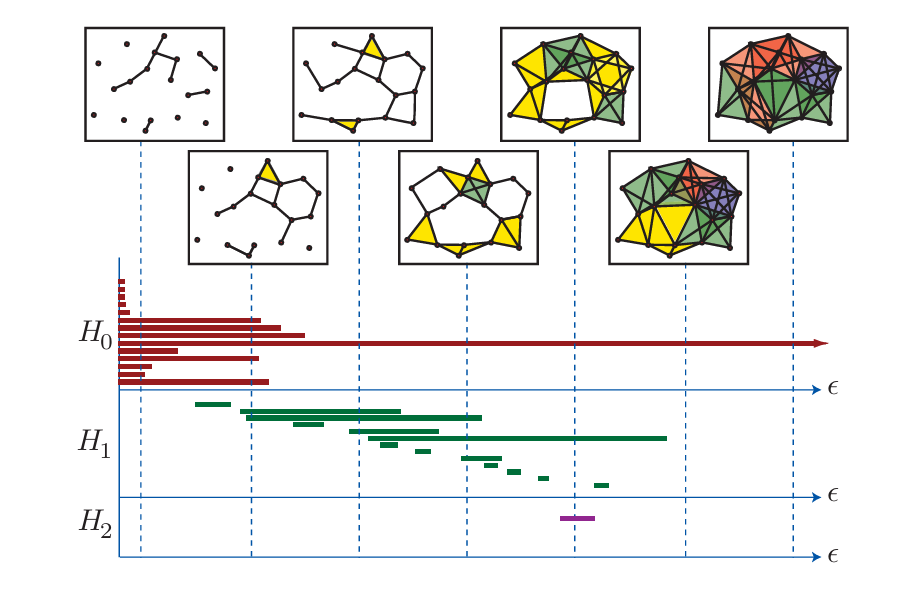
\includegraphics{barcodes robert ghrist.png}
    \caption{\cite{Ghrist2007BarcodesTP}}
    \label{fig:enter-label}
\end{figure}

Displayed below are the persistent diagrams of the homology classes of an annulus, sphere and torus. Each point in the persistence diagram corresponds to a bar in the barcode. The multiplicity of each point is the number of copies of the bar. The distance of the point $(b_i,d_i)_{i \in I}$ to the diagonal line $x=y$ conveys the persistence of the feature. The distance is $d_i - b_i$ and this corresponds to the length of a bar.


\begin{figure}[h!]
  \centering
  \begin{subfigure}{0.8\textwidth}
    \centering
    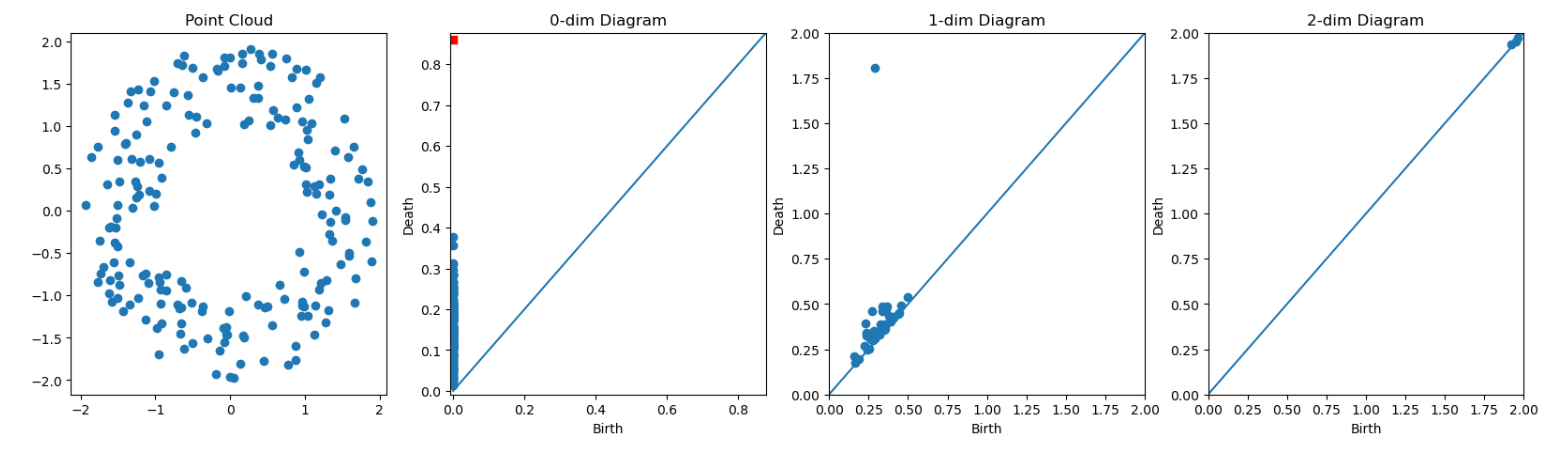
\includegraphics[width=1\linewidth]{Annulus_pt cloud, D-B diagram.png}
    \caption{[Left] Point cloud diagram for an annulus. [Right] The persistence diagram for $H_0, H_1, and H_2$, respectively, of the point cloud annulus.}
    \label{fig:Point cloud of annulus with persistence diagrams for 0,1,2 dimensional persistent homology groups}
  \end{subfigure}
  \begin{subfigure}{0.8\textwidth}
    \centering
    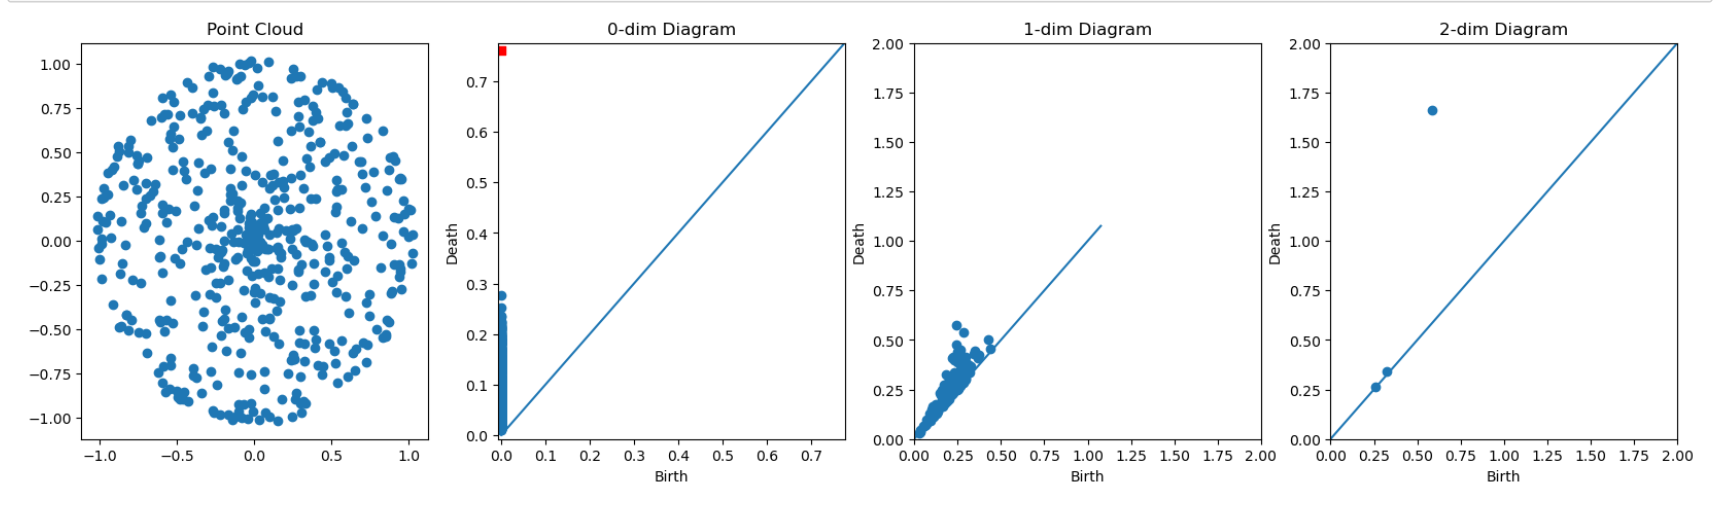
\includegraphics[width=1\linewidth]{Sphere_pt cloud, D-B diagram.png}
    \caption{[Left] Point cloud diagram for a sphere. [Right] The persistence diagram for $H_0, H_1, and H_2$, respectively, of the point cloud sphere.}
    \label{fig:Point cloud of sphere with persistence diagrams for 0,1,2 dimensional persistent homology groups}
    \end{subfigure}
  \begin{subfigure}{0.8\textwidth}
    \centering
    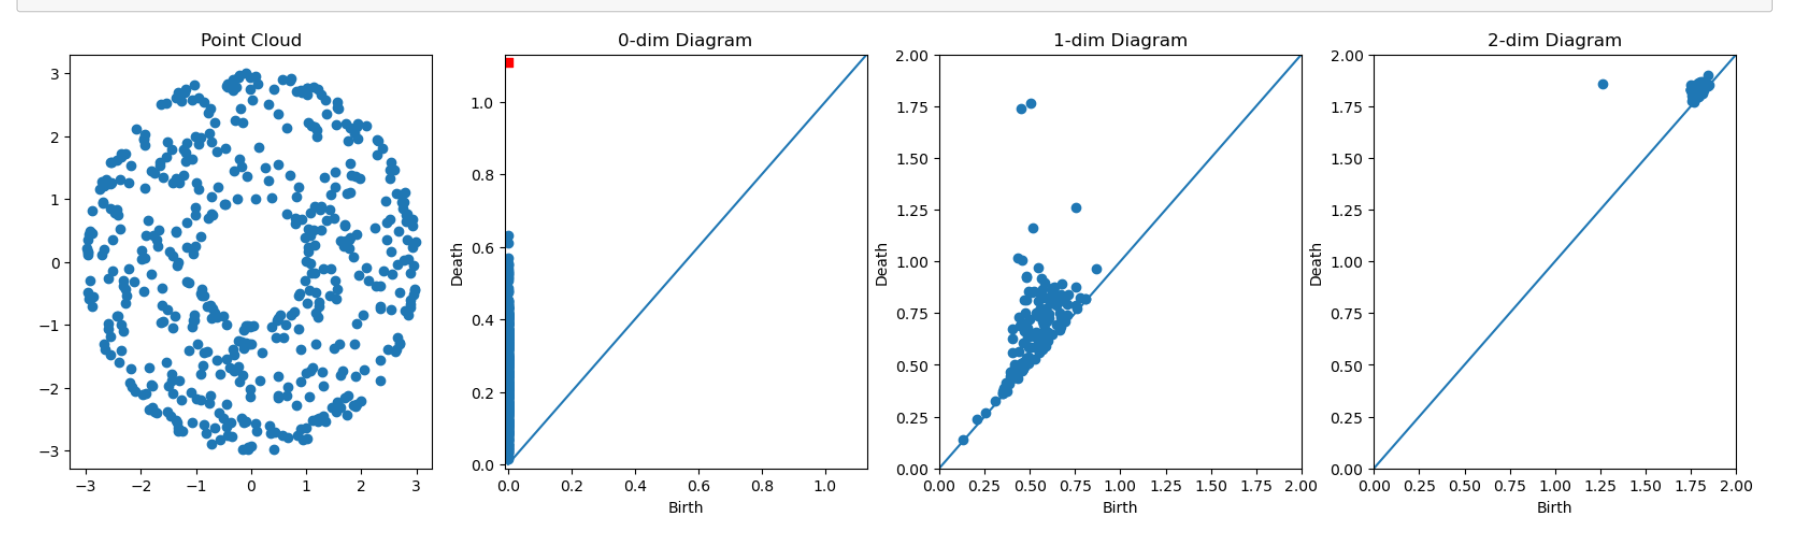
\includegraphics[width =1 \linewidth]{Torus_pt cloud, D-B diagram.png}
    \caption{[Left] Point cloud diagram for a torus. [Right] The persistence diagram for $H_0, H_1, and H_2$, respectively, of the point cloud torus.}
    \label{fig:Point cloud of Torus with persistence diagrams for 0,1,2 dimensional persistent homology groups}
  \end{subfigure}  
\end{figure}


Persistence diagrams convey the same information as a barcode diagram. Also known as birth\ death diagrams, the persistence diagrams shows the time at which a feature appears and disappears as a point instead of a barcode interval. The above diagram serve as a test model for using \textit{ripser}, a python library package, to compute persistent homology. For all point clouds the $H_0$ diagram conveys the birth\ death of connected components hence why there is a red point in the left corner to signify that all the components of the complex connect at the end of the filtration ($\epsilon_{max}$). 
Take the persistence diagram for $H_1$  of the annulus. The $H_1$ homology group quantifies the number of loops or holes in the space. In the $H_1$ diagram, there is a cluser of points near the diagonal line. This indicates that loops appeared in the filtered simplicial complex but disappeared quickly as the difference between birth and death time was short. Those loops did not persist as the filtered complex evolved. However, the point far from the diagonal indicates that this loop persisted while the filtered complex evolved. This is the dominant feature in the $H_1$ homology group. A single loop. This loop correlates to the hole in the middle of the annulus. Nothing interesting is happening in the $H_2$ diagram as the annulus does not have any voids.\\
The $H_1$ diagram for the sphere is also uninteresting as a sphere does not have any loops or holes. Whereas, the $H_2$ diagram for the sphere has one point far away from the diagonal, signifying that there is a prominent void in the sphere which indeed it does.\\
The $H_1$ diagram for the torus has a lot of activity. Many loops are born but soon after disappear with only two dominant loops remaining. These two loops signify the hole in the middle of the torus and the loop around the torus going through the hole. Refer to Fig.\ref{fig:delta-complex structure torus} for the two loops. Finally, the $H_2$ diagram indicates that there is one void in the torus which is true as the torus is a hollow doughnut. \break
In general, points on a persistence diagram that are far from the diagonal indicate the important and dominant features of the filtered simplicial complex. 

\subsection{Wasserstein Distance and Bottleneck Distance}
If data sets are similar, say, we plot the point cloud of an annulus with some noise. Would the persistence diagrams convey the same information or would the dominant features be lost under the noise? The Wasserstein and Bottleneck distance are two methods to compare and quantify the difference in persistence diagrams of different point clouds \cite{bubenik2015statistical}\cite{AZComputePH}\cite{CarlssonTDAappli}. In applications, one can compare the output persistence diagram of a computation from a given dataset to a known model. The Wasserstein and Bottleneck Distance are metrics that compares two persistence diagrams \cite{bubenik2015statistical}.\break

Let $D_{gm_1}$ and $D_{gm_2}$ be two persistence diagrams.
\begin{definition} Let $p \in [1,\infty]$. The $p$th Wasserstein distance between $D_{gm_1}$ and $D_{gm_2}$ is defined by,
\be
W_{p}(D_{gm_1},D_{gm_2}) = \inf\{\Sigma_{x \in D_{gm_1}}d[x, \phi(x)]^p\}^{\frac{1}{p}}
\ee
\end{definition}
To compare two persistence diagrams we need to decide on how to pair points together to take distances between them. As data is often noisy, knowing which points match is difficult. Consider the following;
\begin{definition} A partial matching $\mu$ between two finite sets $X$ and $Y$ is a bijection between two subsets $X' \subseteq X$ and $Y' \subseteq Y$. We call $X'$ the coimage of $\mu$ and $Y'$ the image of $\mu$.
\end{definition}
Before we define the Bottleneck distance recall the supreme norm between two points $\textbf{p}= (p_1,p_2)$ and $\textbf{q}=(q_1,q_2)$ is
\be
||\textbf{p}- \textbf{q}||_{\infty} = \sup\{|p_1 - q_1|, |p_2 - q_2|\}.
\ee
What about the points in the persistence diagram that are not included in the matching? To combat this problem we will define the cost of a partial matching and then the minimised cost over all partial matchings. This takes into consideration the distance of the points from the diagonal.
\begin{definition}The cost of a partial match $\mu$ between $X'$ and $Y'$ is
\be
c(\mu) = \max\{ \sup_{p' \in X'} \{||\textbf{p'}- \mu(\textbf{p'})||_{\infty}\},  \sup_{\{\textbf{p} \in X/X'\}}\{\frac{p_2 - p_1}{2}\}, \sup_{\{\textbf{q} \in Y/Y'\}}\{\frac{q_2 - q_1}{2}\} \}
\ee
\end{definition}

\begin{definition} The bottleneck distance between $D_{gm_1}$ and $D_{gm_2}$ is defined by,
\be
d_B(D_{gm_1} , D_{gm_2}) = \inf\{c(\mu) | \mu , \text{a partial matching} \}
\ee
\end{definition}
The Bottleneck distance defines a metric on persistence diagrams:
\begin{itemize}
    \item $d_B(D_{gm_1} , D_{gm_2}) = 0$ if and only if $D_{gm_1} = D_{gm_2}$.
    \item $d_B(D_{gm_1} , D_{gm_2}) = d_B(D_{gm_2} , D_{gm_1})$.
    \item $d_B(D_{gm_1} , D_{gm_2}) \leq d_B(D_{gm_1} , D_{gm_3}) + d_B(D_{gm_3} , D_{gm_2})$.
\end{itemize}

\subsection{Persistence Landscapes}
However, when analysing data one would like to compute a statistical summary. Persistence landscapes were first introduced in Bubenik \cite{bubenik2015statistical} as an alternative method to display a persistent information. Persistence landscapes are embedding in a Banach space (a vector space) for which statistical and machine learning methods can be easily applied \cite{IntroTDADATAscientists} \cite{bubenik2015statistical}. Persistence landscapes consist a collection of sequences of continuous, piecewise functions $\lambda : \mathbb{N} \times \mathbb{R} \to \mathbb{R}$ that summaries a persistence diagram. \cite{IntroTDADATAscientists}. Essentially, a persistence landscape is a persistence diagram rotated in such a way that the diagonal in the persistence diagram is the x-axis of the persistence landscape. Each birth-death pair $p=(i,j) \in D_{gm}$ is mapped to the point $(\frac{b_i+d_i}{2}, \frac{d_i-b_i}{2})$. Points that lie on the diagonal have been mapped to the x-axis i.e these points are discarded. The sequence of landscape functions is constructed by the tenting of the points in the rotated persistence diagram. For each point p in the persistence diagram the tent function is defined as follows:
\be
\Lambda_{p}(t) =  \begin{cases}
  t - b_i, t \in [b_i, \frac{b_i+d_i}{2}]\\    
  d_i - t, t \in (\frac{b_i+d_i}{2}, d_i] \\
  0,  \text{otherwise}
\end{cases}
\ee
Persistence landscape expresses the summary of the homological features in the form of a collection of piecewise continuous functions. A piecewise continuous function in the persistence landscape is defined for each $k\geq 1$ as 
\be
\lambda_{D_{gm}}(k,t) = k\max \{\Lambda_p(t)\},
\ee
where kmax denotes the kth largest value of the set. If $ k > |I|$ then the value of $k\max$ is zero. Each function $\lambda_{D_{gm}}(k,t)$ is piecewise linear with slope either 0,1 or -1. For someone interested in statistical summary of the dataset the functional space of the persistence landscape representation will prove to be more beneficial \cite{bubenik2015statistical}\cite{https://doi.org/10.1002/jcc.23816}. In the theoretic viewpoint, persistence landscape inherits the same stability properties as persistence diagrams- see \cite{EdelTopPersist}\cite{bubenik2015statistical}\cite{HSchenckAlgebraicFound}. A visualisation of a persistence diagram is shown in Figure\ref{fig:landscape} taken from Bubenik. 

\begin{figure}[h!]
    \centering
    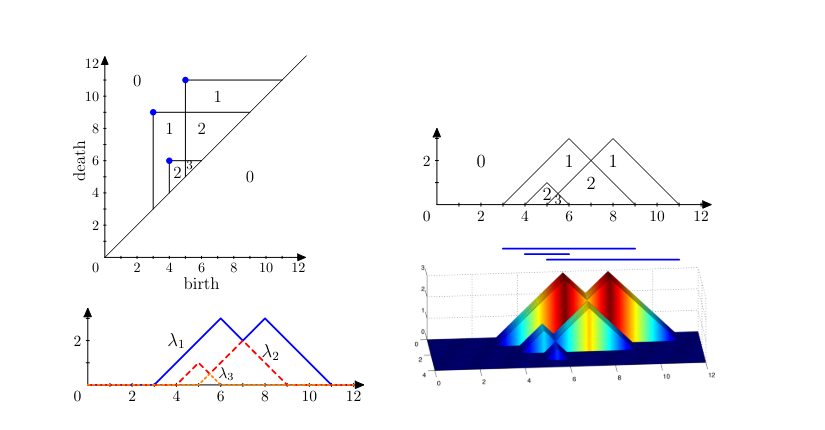
\includegraphics{persistence landscape.png}
    \caption{Persistence landscape diagram taken from Bubenik(2015) \cite{bubenik2015statistical}. Top left diagram contains the three points of the corresponding persistence diagram. Top right diagram is the rotated persistence diagram with the corresponding barcode below. Bottom left diagram is the corresponding persistence landscape and the 3d visualisation in the bottom right.}
    \label{fig:landscape}
\end{figure}



\clearpage
\section{TDA Application to Time Series}
The dataset collected is assumed to lie on the surface of a topological manifold. Topological manifolds are continuous surfaces, hausdorff, paracompact, second countable and locally Euclidean. Prior to analysis, the features of the underlying manifold are unknown. By understanding the topology of the points of the dataset we can extract topological properties about the underlying topological manifold.  Persistent homology is able to identify the features that are invariant under noisy data \cite{smith2020topological}. Data comes in all types of forms and sizes. Topological data analysis has proven great results in image analysis in the medical field but the main focus in this project will be on time series. In the last 10 years, applications of topological data analysis to time series has made progress in the analysis of dynamical systems, time series data and financial data \cite{Gidea2017TopologicalDA}\cite{CarlssonTDAappli}\cite{IntroTDADATAscientists}\cite{ravishanker2019topological}\cite{Umeda2019TopologicalDA} Time series analysis is an extensive field with endless applications in economics, engineering, meteorology, physics, and medicine. Most systems and process that naturally occur in our day to day lives can be thought as a dynamical system. A dynamical system is a time dependant model that describes the evolution of the observed variables \cite{Kuznetsov2023}\cite{dynamicalsystemsHiroki}.These dynamical systems are constantly at play around us and as technology advances so does the immense collection of time series data. Data, in whatever shape and form, is valuable for the predictions of trends and patterns in a desired system. In real life scenarios, mathematical models of dynamical systems are unfortunately not provided for us to compute with. Therefore, data scientists and analysts are solely reliant on the past and current observations of their desired variables. Time series is a sequence of datapoints of observed states collected over time at regular intervals \cite{yap2011stable}. However, the mathematical techniques of persistent homology construct a topological space and study the properties of point cloud datasets. Time series are projections of the observed states not point clouds. The most common approach of reconstruction of time series analysis to a point cloud is the sliding window embedding or also known as Takens embedding theorem \cite{akingbade2023topological}\cite{ravishanker2019topological}\cite{Gidea2017TopologicalDA}\cite{Perea_2014}. This technique involves taking a window neighbourhood of data points; rewrite those points as one vector; map it a higher dimensional space and repeat by sliding the window to create a state-space. State-space reconstruction is a conventional strategy in all fields of mathematics to allow for easier computation.  Takens theorem states that the state-space, a smooth attractor, can be reconstructed from the time series while preserving the topological properties of the original system, and hence provides the perfect opportunity to apply persistent homology \cite{doi:10.1142/S0218127491000634}. 

\subsection{Takens' Embedding Theorem}
A dynamical system is a system in which an event or object changes over time \cite{Kuznetsov2023}. There are many dynamical systems that we encounter in our day to day lives. It is not always possible to have an exact and explicit mathematical description of a dynamical system as most are chaotic; so one has to formulate a mathematical model to approximate the system by observing its variables. The system is described by its variables at a given time and are defined as a state that lives in a space measured by a continuous map called an observation function\cite{DEWOSKIN2010157}. The aim of Takens' Embedding Theorem is to reconstruct an attractor of a dynamical system where an attractor is the space in which most of the states of a dynamical system evolve to \cite{doi:10.1142/S0218127491000634}\cite{ravishanker2019topological}. This approach of converting a time series into a point cloud has been used in the TDA literature to classify time series \cite{Umeda2019TopologicalDA}, quantify periodicity in time series \cite{Perea_2014} and to detect early warning signs for critical transitions \cite{Gidea2017TopologicalDA}\cite{gidea2018topologicalcrypto}.
Let us now formally introduce Takens' embedding theorem. We omit the proof as the proof alone would be suffice to be a project. If the reader wishes to delve into the details refer to...\\

A time series is a sequence of points (observations) indexed by time,
\be
\{x_t\}, t\in T
\ee

\begin{definition} Given a time series $f: t \to \mathbb{R}$, where $t \in T \subset \mathbb{R}$ and a parameter $\tau$, a time-delay embedding is a lift to a time-series $\phi:t\to \mathbb{R}^d$ defined by 
\be
\phi(t) = (f(t), f(t+ \tau),..., f(t + (d-1)\tau))
\ee
\end{definition}

\begin{definition} Let $M$, the state-space, be a compact manifold. A real dynamical system on M is a tuple $(T,M,\psi)$ where $T \subset \mathbb{R}$ is an open interval in the real numbers and $\psi$ is a continuous function $\psi:T \times M \to M$ with $\psi(0,x)=x$ and $\psi(t_2, \psi(t_1,x))= \psi(t_1 +t_2,x)$ for all $x \in M$ and $t_1, t_2 \in T$.
\end{definition}
The state-space $M$ is a discrete or continuous compact manifold that contains all of the possible states of the system. In differential geometry, manifold is a geometric object that generalises the notion of curves, surfaces and higher dimensional spaces. Manifolds are locally Euclidean but globally may have other complex structures such as differentiability, smoothness, connectivity and orientabillity \cite{smoothmanifoldLee}. Each coordinate in the space is a state variable that completely describe the state of the system. The continuous map $\psi$, as defined above, maps point in the state space to other points in the state space and so dictates how these state variables evolve over time. An attractor $A \subset T \times M$ is a compact subset of the state space in which values tend to evolve to and is invariant under $\psi$ \cite{dynamicalsystemsHiroki}. 
Takens' delay embedding provides the conditions under which a attractor can be reconstructed from the observation function \cite{twistytakensPerea}. If we let the map $y:M \to \mathbb{R}$ denote the observation function. We can define for each state $x \in M$ a time series $\phi_x : t \to y \circ \psi(t,x)$ 
\begin{theorem} (Takens' embedding theorem \cite{takens1981detecting}) Let M be a smooth, compact, Riemannian manifold of dimension d. For pairs $(\psi,y)$, with $\psi:M\to M$ is a smooth diffeomorphism and $y:M \to \mathbb{R}$ smooth function, it is a generic property that the $(2d+1)$-delay observation map $\phi_x: M \to \mathbb{R}^{2d+1}$ defined by,
\be
\phi_x = (y(\psi(0,x)), y(\psi(\tau,x)),...,y(\psi(2d\tau,x)))
\ee
is an embedding for all $x \in M$.
\end{theorem}

A smooth, compact, Riemannian manifold, M, is a topological manifold endowed with smooth structures, is closed and bounded and equipped with a Riemannian metric \cite{smoothmanifoldLee}. Smooth structures can be thought as $C^{\infty}$ differentiable structures. The notion of smoothness allows one to do calculus of smooth functions on a manifold. A function $f : U \to V $ where $U \subset \mathbb{R^n}$ open and $V \subset \mathbb{R^m}$ open is said to be smooth if is it has continuous partial derivatives of all order also known as $C^{\infty}$ \cite{smoothmanifoldLee}. If such a smooth function $f$ is bijective and has a smooth inverse functions then $f: U \to V$ is called a diffeomorphism the smooth equivalent to a homeomorphism. A compact manifold is closed and bounded meaning that every sequence converges to a limit point in the manifold. Convergence of sequence can refer to the sequence of a continuous function and so there exists maximum and minimum values of a continuous function; or a sequence of functions $f_n$ converges to a limit function $f$. A Riemannian manifold is a smooth manifold equipped with a Riemannian metric and allows geometric concepts to be defined. A Riemannian metric is an inner product on each tangent space and endows the manifold with a notion of distance, lengths and angles \cite{smoothmanifoldLee}. The ability of distance and lengths is crucial for the construction of a simplicial complex of the embedded time series. The first step to Takens embedding theorem is the time delay map of a given time series. 
An example of a time-delay embedding is the sliding window embedding/algorithm and is commonly used in data analysis and real-time processing of data sets. It is a versatile tool and finds applications in signal processing, data stream processing, machine learning and time series analysis. In the next subchapter the main focus of application will be on  time series and financial time series.
The schematic diagram in Fig.\ref{Sliding Window} depicts a visual for the sliding window embedding of a time series. The process can be thought of as a window of fixed size that slides over the function. At chosen time intervals each window is converted into $2d+1$ dimensional vector and is mapped to a Euclidean space of dimension $2d +1$. Hence for different values of t the sliding window embedding results in a point cloud for f.
\begin{definition} Let $f:\mathbb{R} \to \mathbb{R}$ be a function, $\tau > 0$ a real number and $d>0$ an integer. The sliding window embedding of $f$ based at $t \in \mathbb{R}$, with parameters $d$ and $\tau$, is the vector-valued function given by
\be
\mathbb{SW}_{d,\tau} f : \mathbb{R} \to \mathbb{R}^{2d+1}
\ee
\begin{align}t \rightarrow \begin{bmatrix} f(t)\\ f(t + \tau)\\ f(t+2\tau)\\ \vdots\\
f(t+2d\tau)
\end{bmatrix}
\end{align}
The set $\{\mathbb{SW}_{d,\tau} f(t) | t \in T\}$ is the associated sliding window point cloud.
\end{definition}

\begin{figure}[h!]
    \centering
    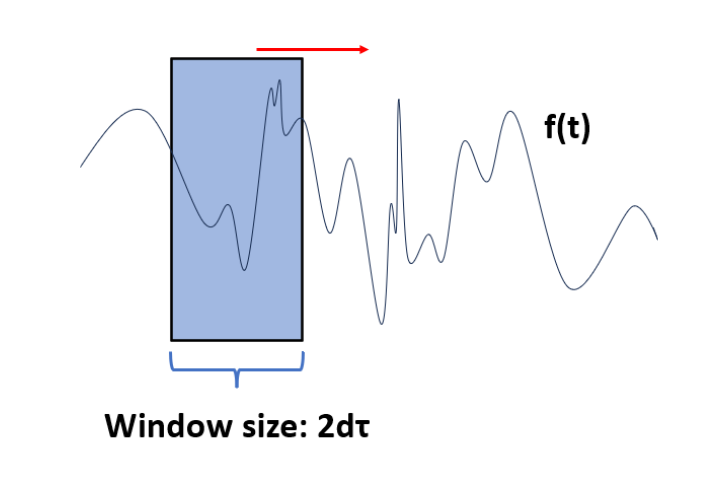
\includegraphics[width = 12cm, height = 8cm]{Sliding_Window.png}
    \caption{Schematic diagram of the sliding window algorithm on a function $f(t)$. The size of the "window" is $2d\tau$, where d is the dimension of the manifold $M$ and $\tau$ is the time delay. The points at discrete times between $t_i$ and $t_{i} + 2d\tau$ are then expressed as a vector in Euclidean space of dimension $2d +1$.} 
    \label{Sliding Window}
\end{figure}
The sliding window embedding is the delay method commonly used in literature and application of TDA \cite{akingbade2023topological}\cite{CSurfaceDataChung}\cite{Umeda2019TopologicalDA}\cite{Gidea2017TopologicalDA}. The embedded space constructed by the sliding window embedding is the desired point cloud of a given time series that recovers the underlying dynamics and geometric structure of the system \cite{twistytakensPerea} \cite{dynamicalsystemsHiroki}.Both the dimension $d$ and the time delay $\tau$ are unknown parameters and are determined in practice \cite{ravishanker2019topological} and determines the number of points in the point cloud. The choice of appropriate time delay and dimension parameters is crucial for the construction of an accurate representation of the time series.\\
\textbf{Time delay parameter}
\begin{itemize}
    \item Autocorrelation function (ACF) $\rho_{\tau}$: ACF is a statistical method used to quantify the correlation between a time series and the time delayed reconstruction. [Truong] chose $\tau$ to be the smallest lag time for which $(\rho_{\tau} - \rho_{\tau -1})/\rho_{\tau} > 1/e$ \cite{ravishanker2019topological}. 
    \item Auto mutual information: Pereira and de Mello \cite{PEREIRA20156026} chose $\tau$ using the first minimum of the auto mutual information \cite{ravishanker2019topological}. Mutual information between the time series and its time delayed reconstruction for different time delay values measures the dependency between the two time series. 
\end{itemize}

\textbf{Dimension}
\begin{itemize}
    \item False nearest neighbours: Calculates the number of false nearest neighbours in the embedded space for range of dimensions. Truong \cite{truong2017exploration} used the false nearest neighbour method \cite{Kennel19923403}. They chose $d$ such that the nearest neighbours of each point in dimension $d$ remain nearest neighbours in dimension $d+1$. 
\end{itemize}



\clearpage

\subsection{TDA on periodic functions}
\begin{figure}[h!]
    \centering
    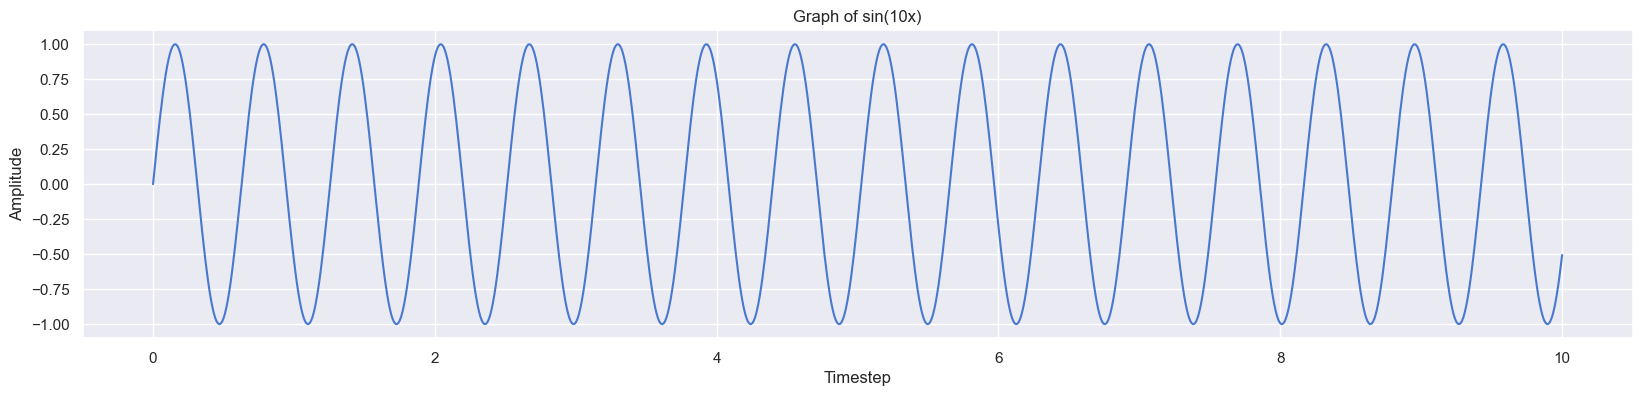
\includegraphics[width = 16cm, height = 6cm]{sin(10x).png}
    \caption{Caption}
    \label{fig:enter-label}
\end{figure}

\begin{figure}[h!]
    \centering
    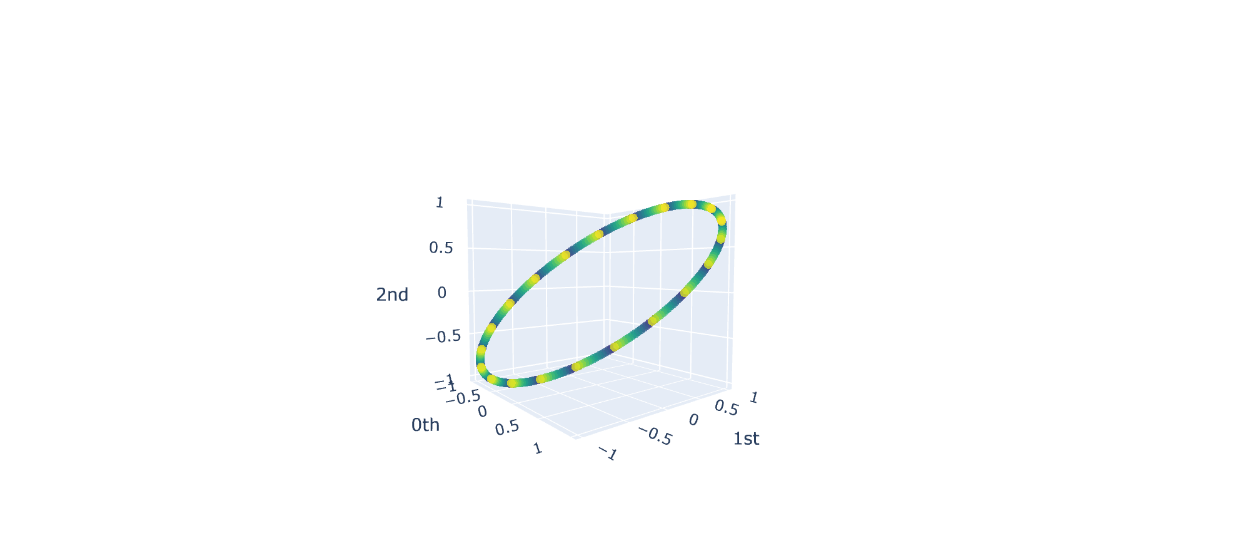
\includegraphics[width=16cm, height=8cm]{pointcloud sin(10x).png}
    \caption{Caption}
    \label{fig:enter-label}
\end{figure}

\begin{figure}[h!]
    \centering
    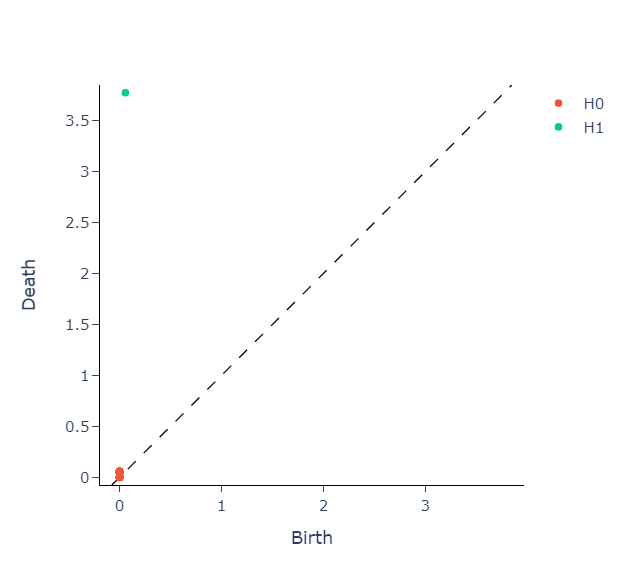
\includegraphics[width= 12cm, height = 8cm]{PD sin(10x).png}
    \caption{Caption}
    \label{fig:enter-label}
\end{figure}

\begin{figure}[h!]
    \centering
    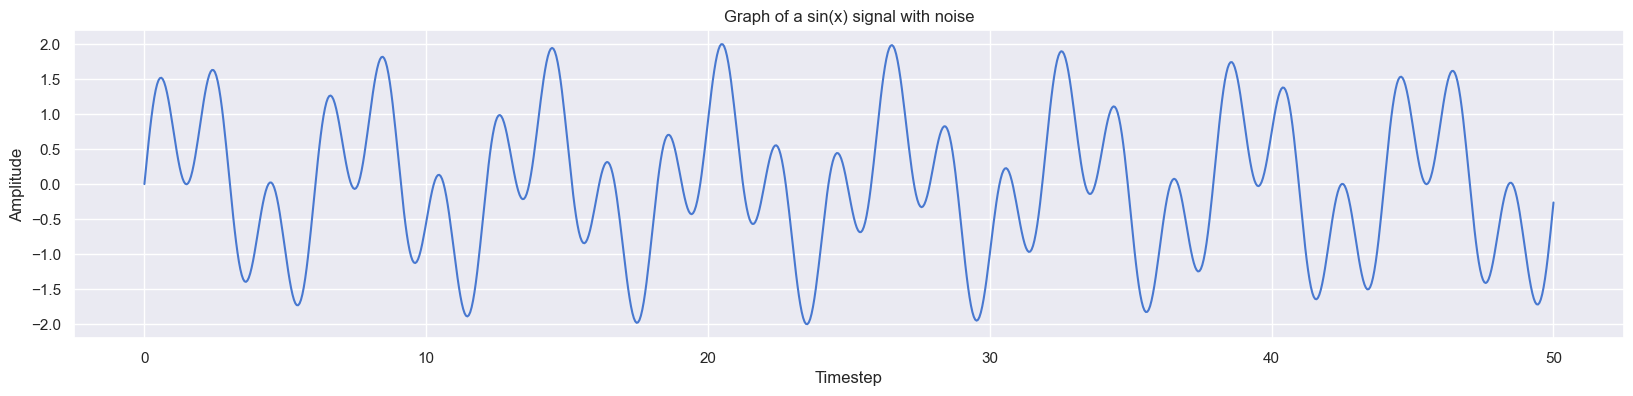
\includegraphics[width= 16cm, height = 8cm]{sin with noise.png}
    \caption{Caption}
    \label{fig:enter-label}
\end{figure}


\begin{figure}[h!]
    \centering
    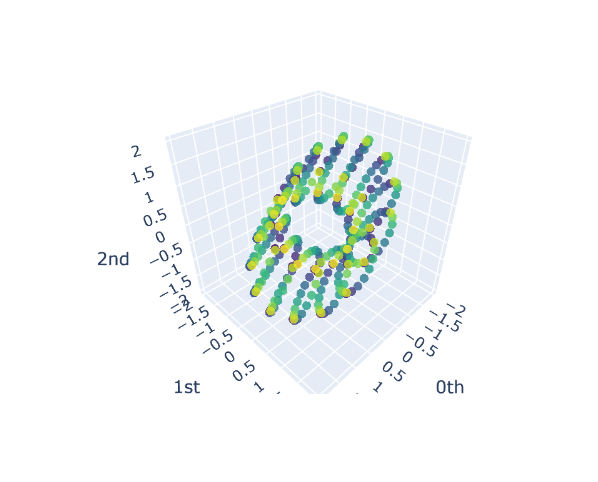
\includegraphics[width= 12cm, height = 6cm]{PC sin with noise.png}
    \caption{Caption}
    \label{fig:enter-label}
\end{figure}

\begin{figure}[h!]
    \centering
    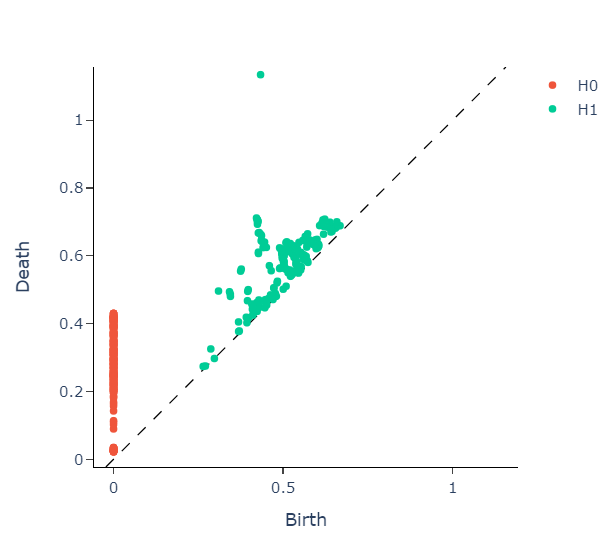
\includegraphics[width= 12cm, height = 8cm]{PD sin with noise.png}
    \caption{Caption}
    \label{fig:enter-label}
\end{figure}


\begin{figure}[h!]
    \centering
    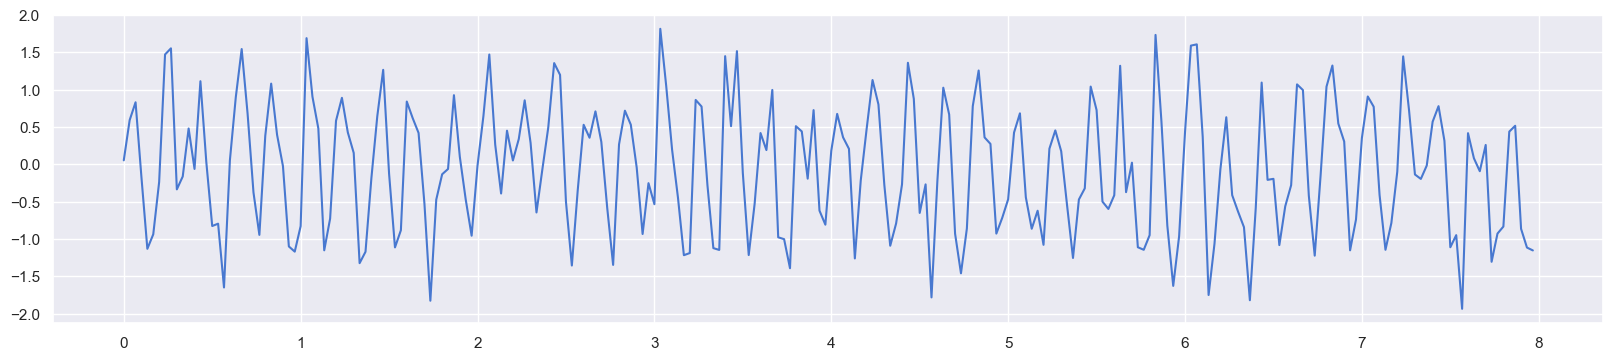
\includegraphics[width= 16cm, height = 7cm]{sin with gaussian noise.png}
    \caption{Caption}
    \label{fig:enter-label}
\end{figure}

\begin{figure}[h!]
    \centering
    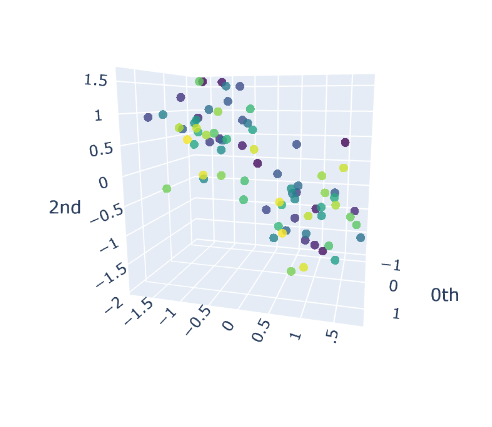
\includegraphics[width= 12cm, height = 8cm]{PC sin w gaussian noise.png}
    \caption{Caption}
    \label{fig:enter-label}
\end{figure}

\begin{figure}[h!]
    \centering
    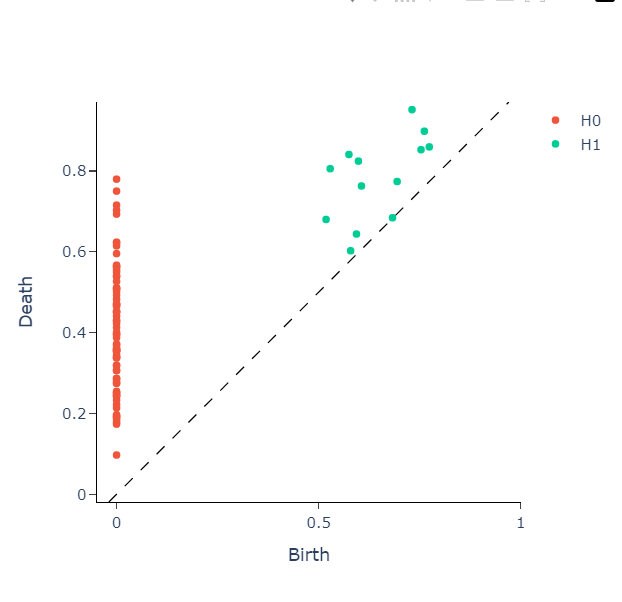
\includegraphics[width= 12cm, height = 8cm]{PD sin with gaussian noise.png}
    \caption{Caption}
    \label{fig:enter-label}
\end{figure}
\clearpage

\subsection{Application to financial time series: Cryptocurrency}
\begin{figure}[h!]
    \centering
    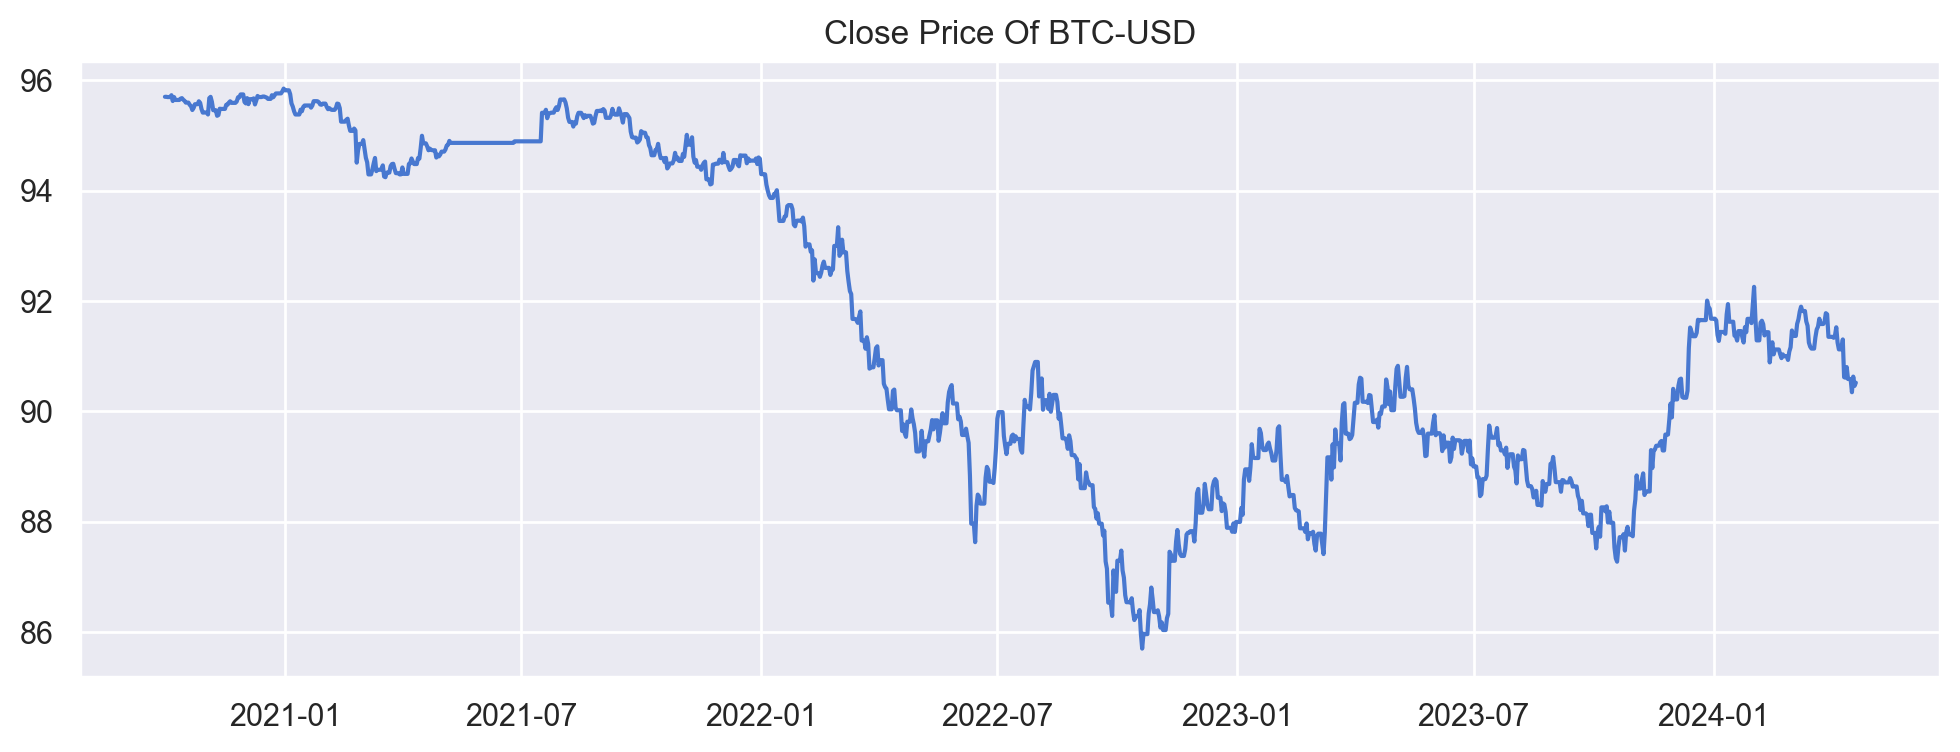
\includegraphics[width= 12cm, height = 8cm]{price BTC.png}
    \caption{Caption}
    \label{fig:enter-label}
\end{figure}


\begin{figure}[h!]
    \centering
    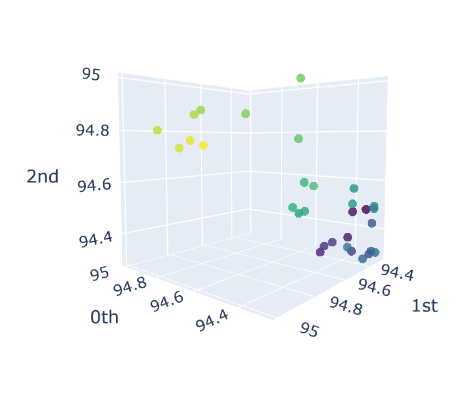
\includegraphics[width= 16cm, height = 8cm]{PC BTC.png}
    \caption{Caption}
    \label{fig:enter-label}
\end{figure}


\begin{figure}[h!]
    \centering
    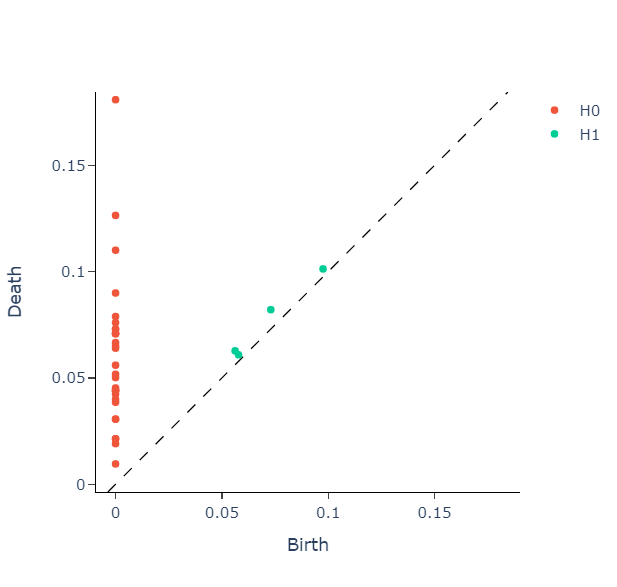
\includegraphics[width= 10cm, height = 8cm]{PD btc.png}
    \caption{Caption}
    \label{fig:enter-label}
\end{figure}
\clearpage

\section{Appendix}
Python code used to generate figures in Chapter. \ref{BARCODES}
\begin{lstlisting}
import numpy as np
import matplotlib.pyplot as plt
import matplotlib.gridspec as gridspec
import networkx as nx
from array import array

import ripser
import persim

import teaspoon.MakeData.PointCloud as makePtCloud
import teaspoon.TDA.Draw as Draw

from teaspoon.SP.network import ordinal_partition_graph
from teaspoon.TDA.PHN import PH_network
from teaspoon.SP.network_tools import make_network
from teaspoon.parameter_selection.MsPE import MsPE_tau
import teaspoon.MakeData.DynSysLib.DynSysLib as DynSysLib

def drawPtCloud(P,diagrams, R=2):
    fig, axes = plt.subplots(nrows=1, ncols=4, figsize=(20,5))
    
    #draw point cloud
    plt.sca(axes[0])
    plt.title('Point Cloud')
    plt.scatter(P[:,0],P[:,1])
    
    #draw diagrams
    plt.sca(axes[1])
    plt.title('0-dim Diagram')
    Draw.drawDgm(diagrams[0])
    
    plt.sca(axes[2])
    plt.title('1-dim Diagram')
    Draw.drawDgm(diagrams[1])
    plt.axis([0,R,0,R])
    
    plt.sca(axes[3])
    plt.title('2-dim Diagram')
    Draw.drawDgm(diagrams[2])
    plt.axis([0,R,0,R])

#Draw annulus point cloud and persistent diagrams
A = makePtCloud.Annulus(N= 200, r=1, R=2, seed = None)
diagrams = ripser.ripser(A, maxdim=2 )['dgms']
drawPtCloud(A,diagrams)

#Draw sphere point cloud and persistent diagrams
S = makePtCloud.Sphere(N=500, r=1, noise=0.02, seed=None)
diagrams= ripser.ripser(S,maxdim=2)['dgms']
drawPtCloud(S,diagrams)

#Draw torus point cloud and persistent diagrams
T =makePtCloud.Torus(N=500, r=1, R=2, seed=None)
diagrams = ripser.ripser(T, maxdim=2)['dgms']
drawPtCloud(T,diagrams)
\end{lstlisting}

\printbibliography[heading = bibintoc,title = {References}]



\end{document}
